\chapter{III-V growth in TASE samples}
\label{chap:growth}

For over a decade, research on monolithic integration of III-V semiconductors has been conducted at \acs{ibm} Research Europe - Zurich. The \acf{tase} method was thought of and developed during this long research effort \cite{borgTASEp2018, Mauthe2021}. \acs{tase} was then applied to integrate emitting and absorbing electronic elements, such as lasing microdisks and nanowire-based photodetectors. As I joined \acs{ibm}, research on both of these device architectures was still ongoing, and, as I was familiarising myself with the tools necessary to conduct my research in the first months of my PhD, I had the opportunity to cooperate with other team members on their projects \cite{Tiwari2021}. Dr. Wen led one such project and aimed to create a single nanowire photodetector. In the end, the project achieved its goal, as seen in \cite{Wen2022}. However, one particular aspect that still needed improvement if the single sample shown in the paper was to be reproducible was the control of the growth front morphology.

Controlling the morphology of the growth front is essential for several reasons. The first is that by ensuring a specific shape of the various heterolayers, the metal-to-semiconductor contact regions can be determined more accurately, aiding in further process steps. The second reason concerns the different integration rates of III group elements on different facets. This was already explored by researchers who showed a marked dependence of the atomic fraction of the III group element in \acs{ingaas} from the facet on which it was grown \cite{Borg2019}.

This chapter expands on the research published by my co-authors and me in \cite{Brugnolotto2023}. The most common crystalline defects observed in \acs{stem_m} images of \acs{tase} grown structures will be discussed to complement this chapter's compositional and morphological introduction. An in-depth exposition of the nanowire design and growth recipes and their analysis, explaining the evolution of the methodology from a simple thick lateral heterostructure to a multi-\acl{qw} architecture with single facet heterointerfaces, follows. When discussing the order of appearance of the wire's internal structure in this thesis, the reference point is set at the \acf{si} seed interface, regardless of its position in the image.

\section{Initial measurements on pre-existing samples}
As the previous section shows, \acs{tase} has been developing for the last decade \cite{Borg2014}. As such, when I started working on the project, an initial study was conducted to determine the crystalline quality of \acs{tase}-grown structures from other ongoing projects. 

\subsection{\texorpdfstring{Defects in \acs{tase} samples}{Defects in TASE samples}}
\label{subsec:pre-existing_samples}

\begin{figure}
    \centering
    \subcaptionbox{Cross section of a multi-seeded coalesced III-V structure grown on Si.
        \label{subfig:SM_overview}
        }{
        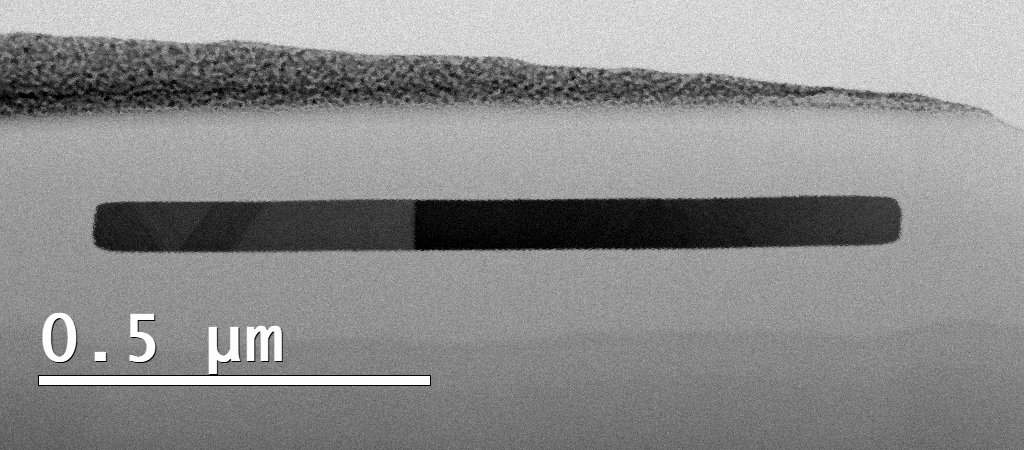
\includegraphics[width = 0.98\textwidth]{3_Growth/2020_Merge/JEOL_BF_150k_SOU76posB_Tunnel5Overview.png
        }
    }
    \subcaptionbox{Detail of twin planes and dislocations.
        \label{subfig:SM_dislocations}
        }{
        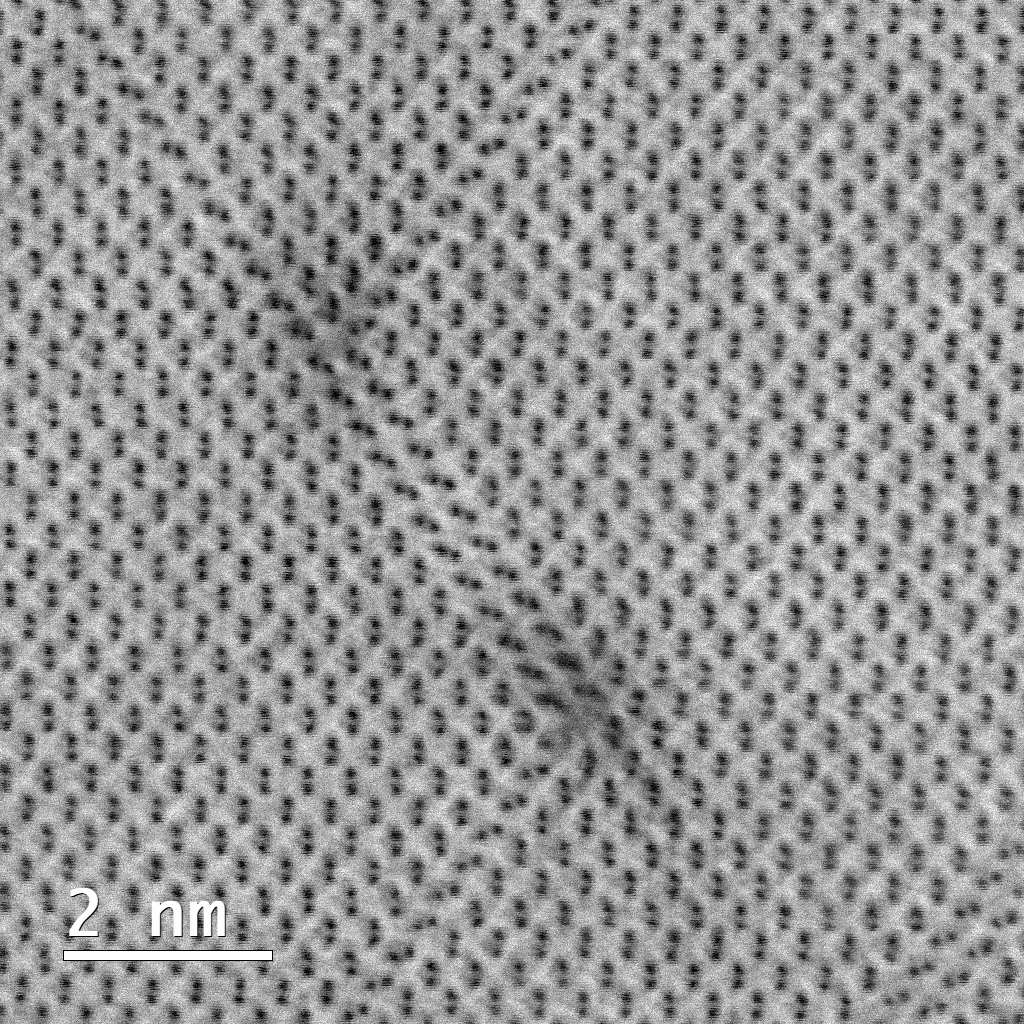
\includegraphics[width = 0.48\textwidth]{3_Growth/2020_Merge/JEOL_BF_20M_SOU76posB_Tunnel5Seed1DefectMeet1.png
        }
    }
    \subcaptionbox{Detail of a grain boundary.
        \label{subfig:SM_merge_position}
        }{
        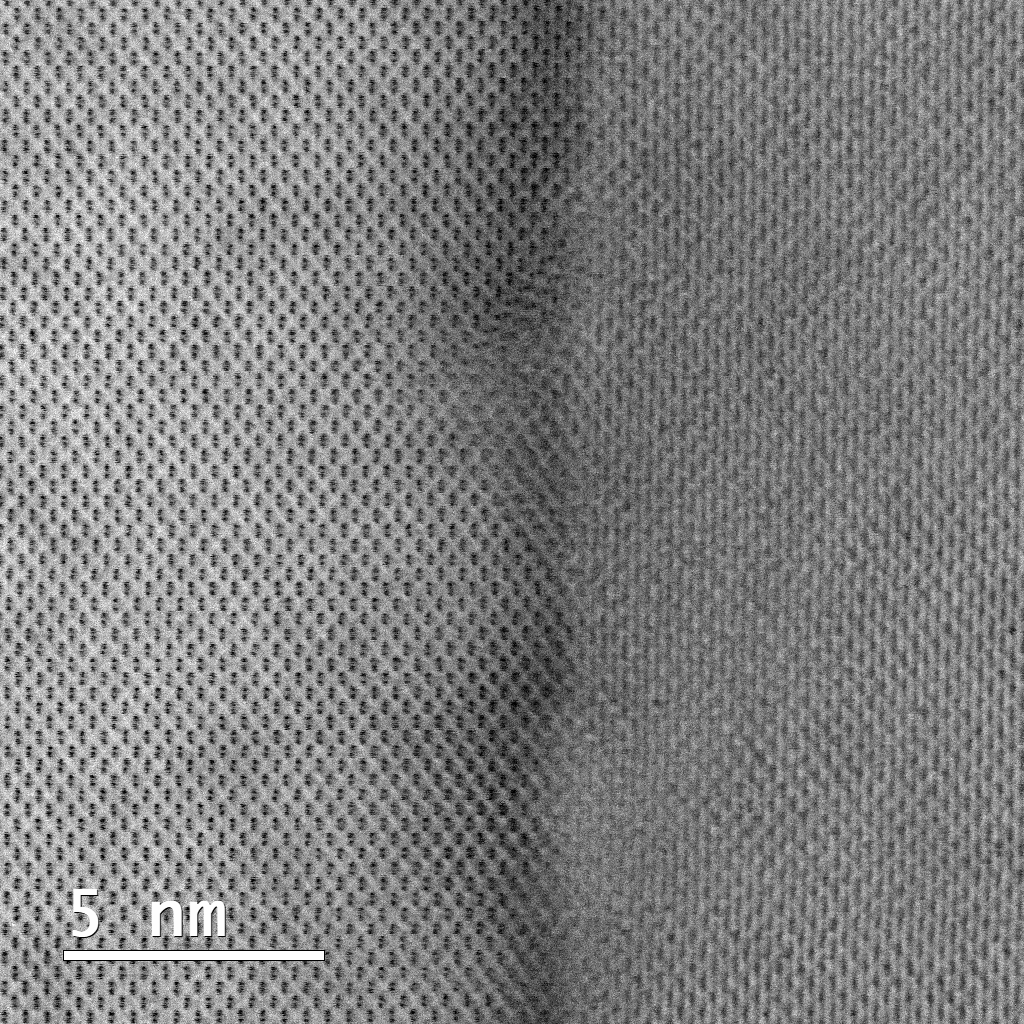
\includegraphics[width = 0.48\textwidth]{3_Growth/2020_Merge/JEOL_BF_10_M_SOU76posB_Tunnel5_Boundary_Seeds_2_3.png
        }
    }
    \caption[\acs{bf}-\acs{stem_m} images of a cross section perpendicular to the growth direction of a \acs{tase} structure.]{\acs{bf}-\acs{stem_m} images of a cross section of a \acs{tase} structure. \subref{subfig:SM_overview} overview image of the entire platelet. Two regions can be identified in this image, with the leftmost area of the left section presenting an area with darker lines describing a "v" shape. These lines are caused by \acs{rtp}s. \subref{subfig:SM_dislocations} a pair of stair-rod dislocations \cite{Bologna2018} imaged in high-resolution. \subref{subfig:SM_merge_position} high-resolution image of the area in which the two regions in \subref{subfig:SM_overview} meet.}
    \label{fig:2020_Merge}
\end{figure}

\Acl{rtp}s (\acs{rtp}s) were found to be the most common crystalline defect from the characterisation conducted on \acs{tase}-grown samples throughout the project. A widespread presence of micro twins was found in all samples \cite{Brugnolotto2023, Brugnolotto2023_2}, even those dating to before the start of the project \cite{Staudinger2018}. Only one of the structures, created by merging different nanowires into a larger platelet, had dislocations (Figure~\ref{subfig:SM_dislocations}). 
\par
The sample in Figure~\ref{fig:2020_Merge} was grown by Svenja Mauthe before the beginning of my stay at \acs{ibm} Research Europe - Zurich as part of her study on the controlled introduction of dislocation at the merging point of two growing crystals \cite{Mauthe2021}. A cross-section of a structure deriving from one such experiment is shown in Figure~\ref{subfig:SM_overview}. This lamella was cut in the area of the device where the wires had already merged. Two areas of the structure stand out particularly: on the left side of the image, a series of "v-shaped" parallel lines denote the presence of two-fold \acf{rtp}s in orthogonal \hkl{111} planes. In this region, Figure~\ref{subfig:SM_dislocations} shows the two stair-rod dislocations forming where two twin planes intersect or when one is annihilated and the other changes direction. This type of defect was the subject of an in-depth study by Bologna et al. \cite{Bologna2018}, but it will not make another appearance in any of the other \acf{stem_m} images recorded during my studies. However, it should be noted that the vast majority of cross sections imaged from this point on were cut along the growth axis instead of perpendicularly to it as this one was. Figure~\ref{subfig:SM_merge_position} shows the interface between the light grey and dark grey segments that comprise the III-V crystal in Figure~\ref{subfig:SM_overview}. 
\par
As made clear by the definition with which the atomic columns are visible on the left-hand side of Figure~\ref{subfig:SM_merge_position} the sample was orientated to achieve the channelling condition of the \acs{stem_m} electron beam in the corresponding crystal. The crystal's lattice on the right-hand side of the same image does not appear as clearly defined: a slight rotation at the time of nucleation might have happened for one of the two seeds pictured. Of course, since the platelet originated from five different seeds, an empirical assumption can be made about two of them prevailing over the other three. This hypothesis is further supported by the presence of \acs{rtp}s on the leftmost portion of the crystalline slice in Figure~\ref{subfig:SM_overview}. At the same time, the area to its immediate right does not show signs of \acs{rtp}s, hinting at the possibility of growth developing in two different directions. 

\section{\texorpdfstring{Fabrication on \acs{si}\hkl(0 0 1) \acs{soi}}{Fabrication on Si(001) SOI}}

\begin{figure}
    \centering
    \subcaptionbox{
    \hkl(0 0 1) in-plane crystalline directions.
    \label{subfig:001wafer_directions}
    }{
        \tikzsetnextfilename{001wafer_directions}
        \begin{tikzpicture}
            \begin{scope}[scale=0.22]
                \draw (45:11cm) -- (45:13cm);
                \draw[stealth-stealth] (45:12cm) arc [start angle = 45, end angle = -45, radius = 12cm] node[midway, anchor = west]{\qty{90}{\degree}};
                \draw (-45:11cm) -- (-45:13cm);
                \draw (-45:10cm) arc [start angle=315, end angle=358.8, radius=10cm] -- (9.8935cm,-1.065mm) arc [start angle=-135, end angle=-225, radius=1.5mm] -- (9.9987cm,2.13mm) arc [start angle=1.20, end angle=45, radius=10cm];
                \draw[dashed] (45:10cm) arc [start angle=45, end angle=315, radius=10cm];
                \path[decorate,decoration={text along path, text={Repeated by symmetry},text align=center}] (315:11) arc [start angle=315,end angle=45,radius=11];
                \draw[dashed] (45:10cm) -- (0, 0) -- (-45:10cm);
                \draw[-stealth, thick] (0, 0) node[anchor=east] {\hkl[0 0 1]} -- ++ (0:4cm) node[anchor=west] {\hkl[1 1 0]};
                \draw[-stealth, thick] (0, 0) -- ++ (45:4cm) node[anchor=south east] {\hkl[0 1 0]};
                \draw[-stealth, thick] (0, 0) -- ++ (315:4cm) node[anchor=north east] {\hkl[1 0 0]};
                \node[mark size=2pt] at (0, 0) {\pgfuseplotmark{square*}};
            \end{scope}
        \end{tikzpicture}
    }
    \subcaptionbox{
    Microstructure designs.
    \label{subfig:enterprise_design}
    }{
        \tikzsetnextfilename{enterprise_design}
        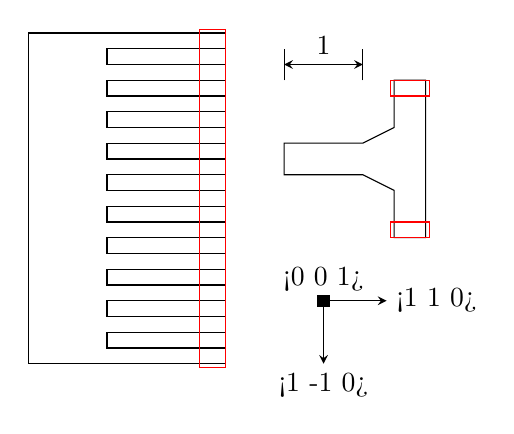
\begin{tikzpicture}
            \begin{scope}[scale=0.1]
                \draw (20, 1) -- ++ (10, 0) -- ++ (-26.6:4.445) -- ++ (0, -6) -- ++ (4, 0) -- ++ (0, 20) -- ++ (-4, 0) -- ++ (0, -6) -- ++ (26.6:-4.445) -- ++ (-10, 0) -- cycle;
                \draw[red] (33.5, 11) rectangle (38.5, 13);
                \draw[red] (33.5, -7) rectangle (38.5, -5);
                \draw (-12.5, -23) -- ++ (25, 0) -- ++ (0,2) -- ++ (-15, 0) -- ++ (0, 2) -- ++ (15, 0) -- ++ (0,2) -- ++ (-15, 0) -- ++ (0, 2) -- ++ (15, 0) -- ++ (0,2) -- ++ (-15, 0) -- ++ (0, 2) -- ++ (15, 0) -- ++ (0,2) -- ++ (-15, 0) -- ++ (0, 2) -- ++ (15, 0) -- ++ (0,2) -- ++ (-15, 0) -- ++ (0, 2) -- ++ (15, 0) -- ++ (0,2) -- ++ (-15, 0) -- ++ (0, 2) -- ++ (15, 0) -- ++ (0,2) -- ++ (-15, 0) -- ++ (0, 2) -- ++ (15, 0) -- ++ (0,2) -- ++ (-15, 0) -- ++ (0, 2) -- ++ (15, 0) -- ++ (0,2) -- ++ (-15, 0) -- ++ (0, 2) -- ++ (15, 0) -- ++ (0,2) -- ++ (-15, 0) -- ++ (0, 2) -- ++ (15, 0) -- ++ (0,2) -- ++ (-25, 0) -- cycle;
                \draw[red] (9.2, -23.5) rectangle (12.5, 19.5);
                \draw[stealth-stealth] (20, 15) -- (30, 15) node [midway, anchor = south] {\qty{1}{\micro\metre}};
                \draw (20, 13) -- (20, 17);
                \draw (30, 13) -- (30, 17);
                \draw[-stealth] (25cm, -15cm) node[anchor=south] {\hkl<0 0 1>} -- ++ (-90:8cm) node[anchor=north] {\hkl<1 -1 0>};
                \draw[-stealth] (25cm, -15cm) -- ++ (0:8cm) node[anchor=west] {\hkl<1 1 0>};
                \node[mark size=2pt] at (25, -15) {\pgfuseplotmark{square*}};
            \end{scope}
        \end{tikzpicture}
    }
    \subcaptionbox{
    \acs{si} seed area before growth.
    \label{subfig:enterprise_etchback}
    }{
        \tikzsetnextfilename{enterprise_etchback}
        \begin{tikzpicture}
            \filldraw[fill=Si_green] (2cm, 0cm) -- (2cm, 22mm) -- (3.5cm, 22mm) -- ++ (-54.7:2.8cm) node[midway, anchor=west]{\rotatebox{-54.7}{\hkl{1 1 1}}} --  node[midway, anchor=south] {\acs{si}} cycle;
            \filldraw[fill=SiO2_blue] (0cm, -10mm) -- (10cm, -10mm) -- (10cm, 0cm) -- (2cm, 0mm)-- (2cm, 22mm) -- (10cm, 22mm) -- (10cm, 32mm) -- (0cm, 32mm) --  node[midway, anchor=west] {\acs{sio2}} cycle; 
            \draw (3.2cm, 22mm) arc [start angle = 180, end angle = 324.7, radius = 3mm] node[midway, anchor = north east]{\qty{125.3}{\degree}};
            \draw[-stealth] (8cm, 7mm) node[anchor=north] {\hkl<1 -1 0>} -- ++ (90:0.8cm) node[anchor=south] {\hkl<0 0 1>};
            \draw[-stealth] (8cm, 7mm) -- ++ (0:0.8cm) node[anchor=west] {\hkl<1 1 0>};
            \node[mark size=2pt] at (8, 7mm) {\pgfuseplotmark{diamond*}};
        \end{tikzpicture}
    }
    \caption[\hkl(0 0 1) \acs{soi} wafer symmetry and microstructure design.]{Wafer symmetry and microstructure design. \subref{subfig:001wafer_directions} shows the in-plane low-index crystalline directions in a \hkl(0 0 1) wafer, using a \qty{90}{\degree} arc centred around the notch that indicates the in-plane direction \hkl[1 1 0]. The rest of the directions can be deduced by the symmetry defined by the four-fold axis perpendicular to the wafer plane. \subref{subfig:enterprise_design} illustrates two different microstructure designs, complemented by a scale bar and an in-plane orientation guide. The black designs were transferred to the device \acs{si} layer of the \acs{soi} wafer, while the red designs marked the position of the template openings. \subref{subfig:enterprise_etchback} is a drawing of the \acs{si} seed area showing its configuration after etch-back for a structure orientated along an in-plane \hkl<1 1 0> direction.}
    \label{fig:001_Templat5e_Design}
\end{figure}

Nanofabrication was carried out with the \acs{tase} process (see \autoref{chap:tase} for details) and, together with the later sample characterisation, took place in highly controlled environments such as a cleanroom and noise-free lab (see \autoref{chap:tools}). Firstly, the shape of the ensemble of nucleation seed and nanostructure is transferred to the \acl{si} device layer of the \acs{soi} wafer through a series of lithographic and etching steps. The template, composed of \acs{sio2}, is then deposited on top of the resulting microstructures. Finally, the template is opened in one or more positions before the etch-back of the sacrificial \acl{si} volume and the introduction of \acf{mocvd} grown III-V semiconductor in its place \cite{Schmid2015, borgTASEp2018}.
\par
Initial growth experiments focussed on nanowires, one of the simplest geometries. The relative simplicity of the nanowires allows for the study of the impact of even minor modifications of the growth recipes on the final crystal, both in terms of structure and composition.

\subsection{Template design considerations}

The orientation of the \acs{tase} template on the \acl{si} \hkl(0 0 1) surface, and therefore the crystalline direction along which the growth will take place, is the first key factor in determining the final shape of the crystal. In the \acl{si} space group \num{227} \cite{osti_si}, the \hkl<0 0 1> vector contains a four-fold axis, represented by a square dot in Figure~\ref{subfig:001wafer_directions}. If we were to examine the possible in-plane directions within an arbitrary \qty{90}{\degree} angle, we would find them repeated three more times in the remaining in-plane \qty{270}{\degree} arc because of this symmetry element. Figure~\ref{subfig:001wafer_directions} shows this principle applied to the \hkl(0 0 1) wafer used to fabricate the first samples. By drawing a \qty{90}{\degree} angle around the notch indicating the \hkl[1 1 0] direction and highlighting the low-index in-plane directions, the two equivalent \hkl[0 1 0] and \hkl[1 0 0] directions define the edges of the arc. Although the cubic III-V semiconductor phase is zincblende (space group \num{216}) \cite{wyckoff1963crystal, osti_gaas_zb, osti_inas_zb, osti_inp_zb}, equivalent symmetry considerations can be made, provided the polar nature of the compound is taken into account.
\par
Most previous \acs{tase} nanowire growth experiments have used the \hkl<1 1 0> vector as the primary in-plane growth axis \cite{Brunelli2019, Knoedler2017, Borg2017, Schmid2015}. Therefore, this direction was selected as a starting point to analyse the growth results. Figure~\ref{subfig:enterprise_design} shows the two designs divided by colour in the two \acf{ebl} exposures during fabrication with scale and direction relative to the crystal. For the first design, the black pattern comprises a series of \num{11} nanowires and a back anchor in a comb-like structure. These, while maintaining a constant wire length, were designed in multiple wire widths ranging from \qty{50}{\nano\metre} to \qty{500}{\nano\metre}. In contrast, the second design is shaped as a capital "T" with a wire thickness ranging from \qty{50}{\nano\metre} to \qty{400}{\nano\metre}. These designs are transferred onto the \acl{si} layer by selectively etching the superfluous material around them. Subsequently, the resulting structures are encapsulated in a \acs{sio2} layer that forms the template. \acs{ebl} is then used to define the area of the template to be opened (in red in Figure~\ref{subfig:enterprise_design}).
\par
Figure~\ref{subfig:enterprise_etchback} shows the situation of the \acl{si} seed of one of the nanowires after template opening and etch-back of the microstructured \acl{si} device layer. It is encased on all but one side by the oxide template and the buried oxide. It presents a surface composed of one (or, as seen experimentally, two, with one being larger than the other in most seed surfaces) \hkl{1 1 1} facets because of the chemistry of the \acs{tmah} etch, which is slower on this densely-packed facet \cite{Zubel2012}. The acute angle that this type of facet forms with the template can easily result in unwanted effects, such as incomplete template filling in the seed area \cite{Scherrer2022}. 

\subsection{Simple precursor switching sequence}

\begin{figure}
    \centering
    \subcaptionbox{
    Growth recipe \cite{Brugnolotto2023}.
    \label{subfig:recipe1}
    }{
        \tikzsetnextfilename{recipe1}
    \begin{tikzpicture}
    \begin{scope}
    % lines
        \node [label={[label distance=0]180:\acs{in}}] at (0, 0) {};
        \draw [cb1_orange, ultra thick] (0, 0) -- (4.2, 0);
        \draw [cb1_dark_blue, ultra thick] (4.2, 0) -- (6.6, 0);
        \node [label={[label distance=0]180:\acs{ga}}] at (0, -0.5) {};
        \draw [cb1_orange, ultra thick] (0, -0.5) -- (4.2, -0.5cm);
        \node [label={[label distance=0]180:\acs{as}}] at (0, -1) {};
        \draw [cb1_orange, ultra thick] (0, -1) -- (4.2, -1);
        \node [label={[label distance=0]180:\acs{p}}] at (0, -1.5) {};
        \draw [cb1_dark_blue, ultra thick] (4.2, -1.5) -- (6.6, -1.5);
    % labels and markers for the timescale
        \node [label={[label distance=0]180:Time (\second)}] at (0, -2) {};
        \draw [-stealth] (0, -2) -- (6.9, -2);
        \draw [] (0, 0.2) -- (0, -2.2) node[anchor = north] {\num{0}};
        \draw [] (4.2, 0.2) -- (4.2, -2.2) node[anchor = north] {\num{420}};
        \draw [] (6.6, 0.2) -- (6.6, -2.2) node[anchor = north] {\num{660}};
    \end{scope}
    \begin{scope} [shift={(8cm, -0.5)}]
        \draw [cb1_orange, ultra thick] (0, 0) -- (0.5, 0) node[anchor = west, text=black] {\acs{ingaas}};
        \draw [cb1_dark_blue, ultra thick] (0, -0.5) -- (0.5, -0.5) node[anchor = west, text=black] {\acs{inp}};
        \draw (-0.5, 0.5) -- (2.5, 0.5) -- (2.5, -1.15) -- node[midway, fill=white] {Legend} (-0.5, -1.15) -- cycle;
    \end{scope}
    %\begin{scope}[yshift = -4cm]
    %    \node [label={[label distance=0cm]180:\acs{in}}] at (0, 0) {};
    %    \draw [cb1_orange, ultra thick] (0, 0) -- (20cm, 0);
    %    \node [label={[label distance=0cm]180:\acs{ga}}] at (0, -0.5cm) {};
    %    \draw [cb1_orange, ultra thick] (0, -0.5cm) -- (20cm, -0.5cm);
    %    \node [label={[label distance=0cm]180:\acs{as}}] at (0, -1cm) {};
    %    \draw [cb1_orange, ultra thick] (0, -1cm) -- (20cm, -1cm);
    %    \node [label={[label distance=0cm]180:\acs{p}}] at (0, -1.5cm) {};
    %    \draw [cb1_orange, ultra thick] (0, -1.5cm) -- (20cm, -1.5cm);
    %    \node [label={[label distance=0cm]180:Time (\second)}] at (0, -2.5cm) {};
    %    \draw [black, -stealth] (0, -2.5cm) -- (20cm, -2.5cm);
    %\end{scope}
    \end{tikzpicture}
    }
    \subcaptionbox{
    \qty{52}{\degree} tilted image of III-V nanowires.
    \label{subfig:comb_sample1}
    }{
        \tikzsetnextfilename{comb_sample1}
    \begin{tikzpicture}
        \node[inner sep=0pt] (image) at (0,0) {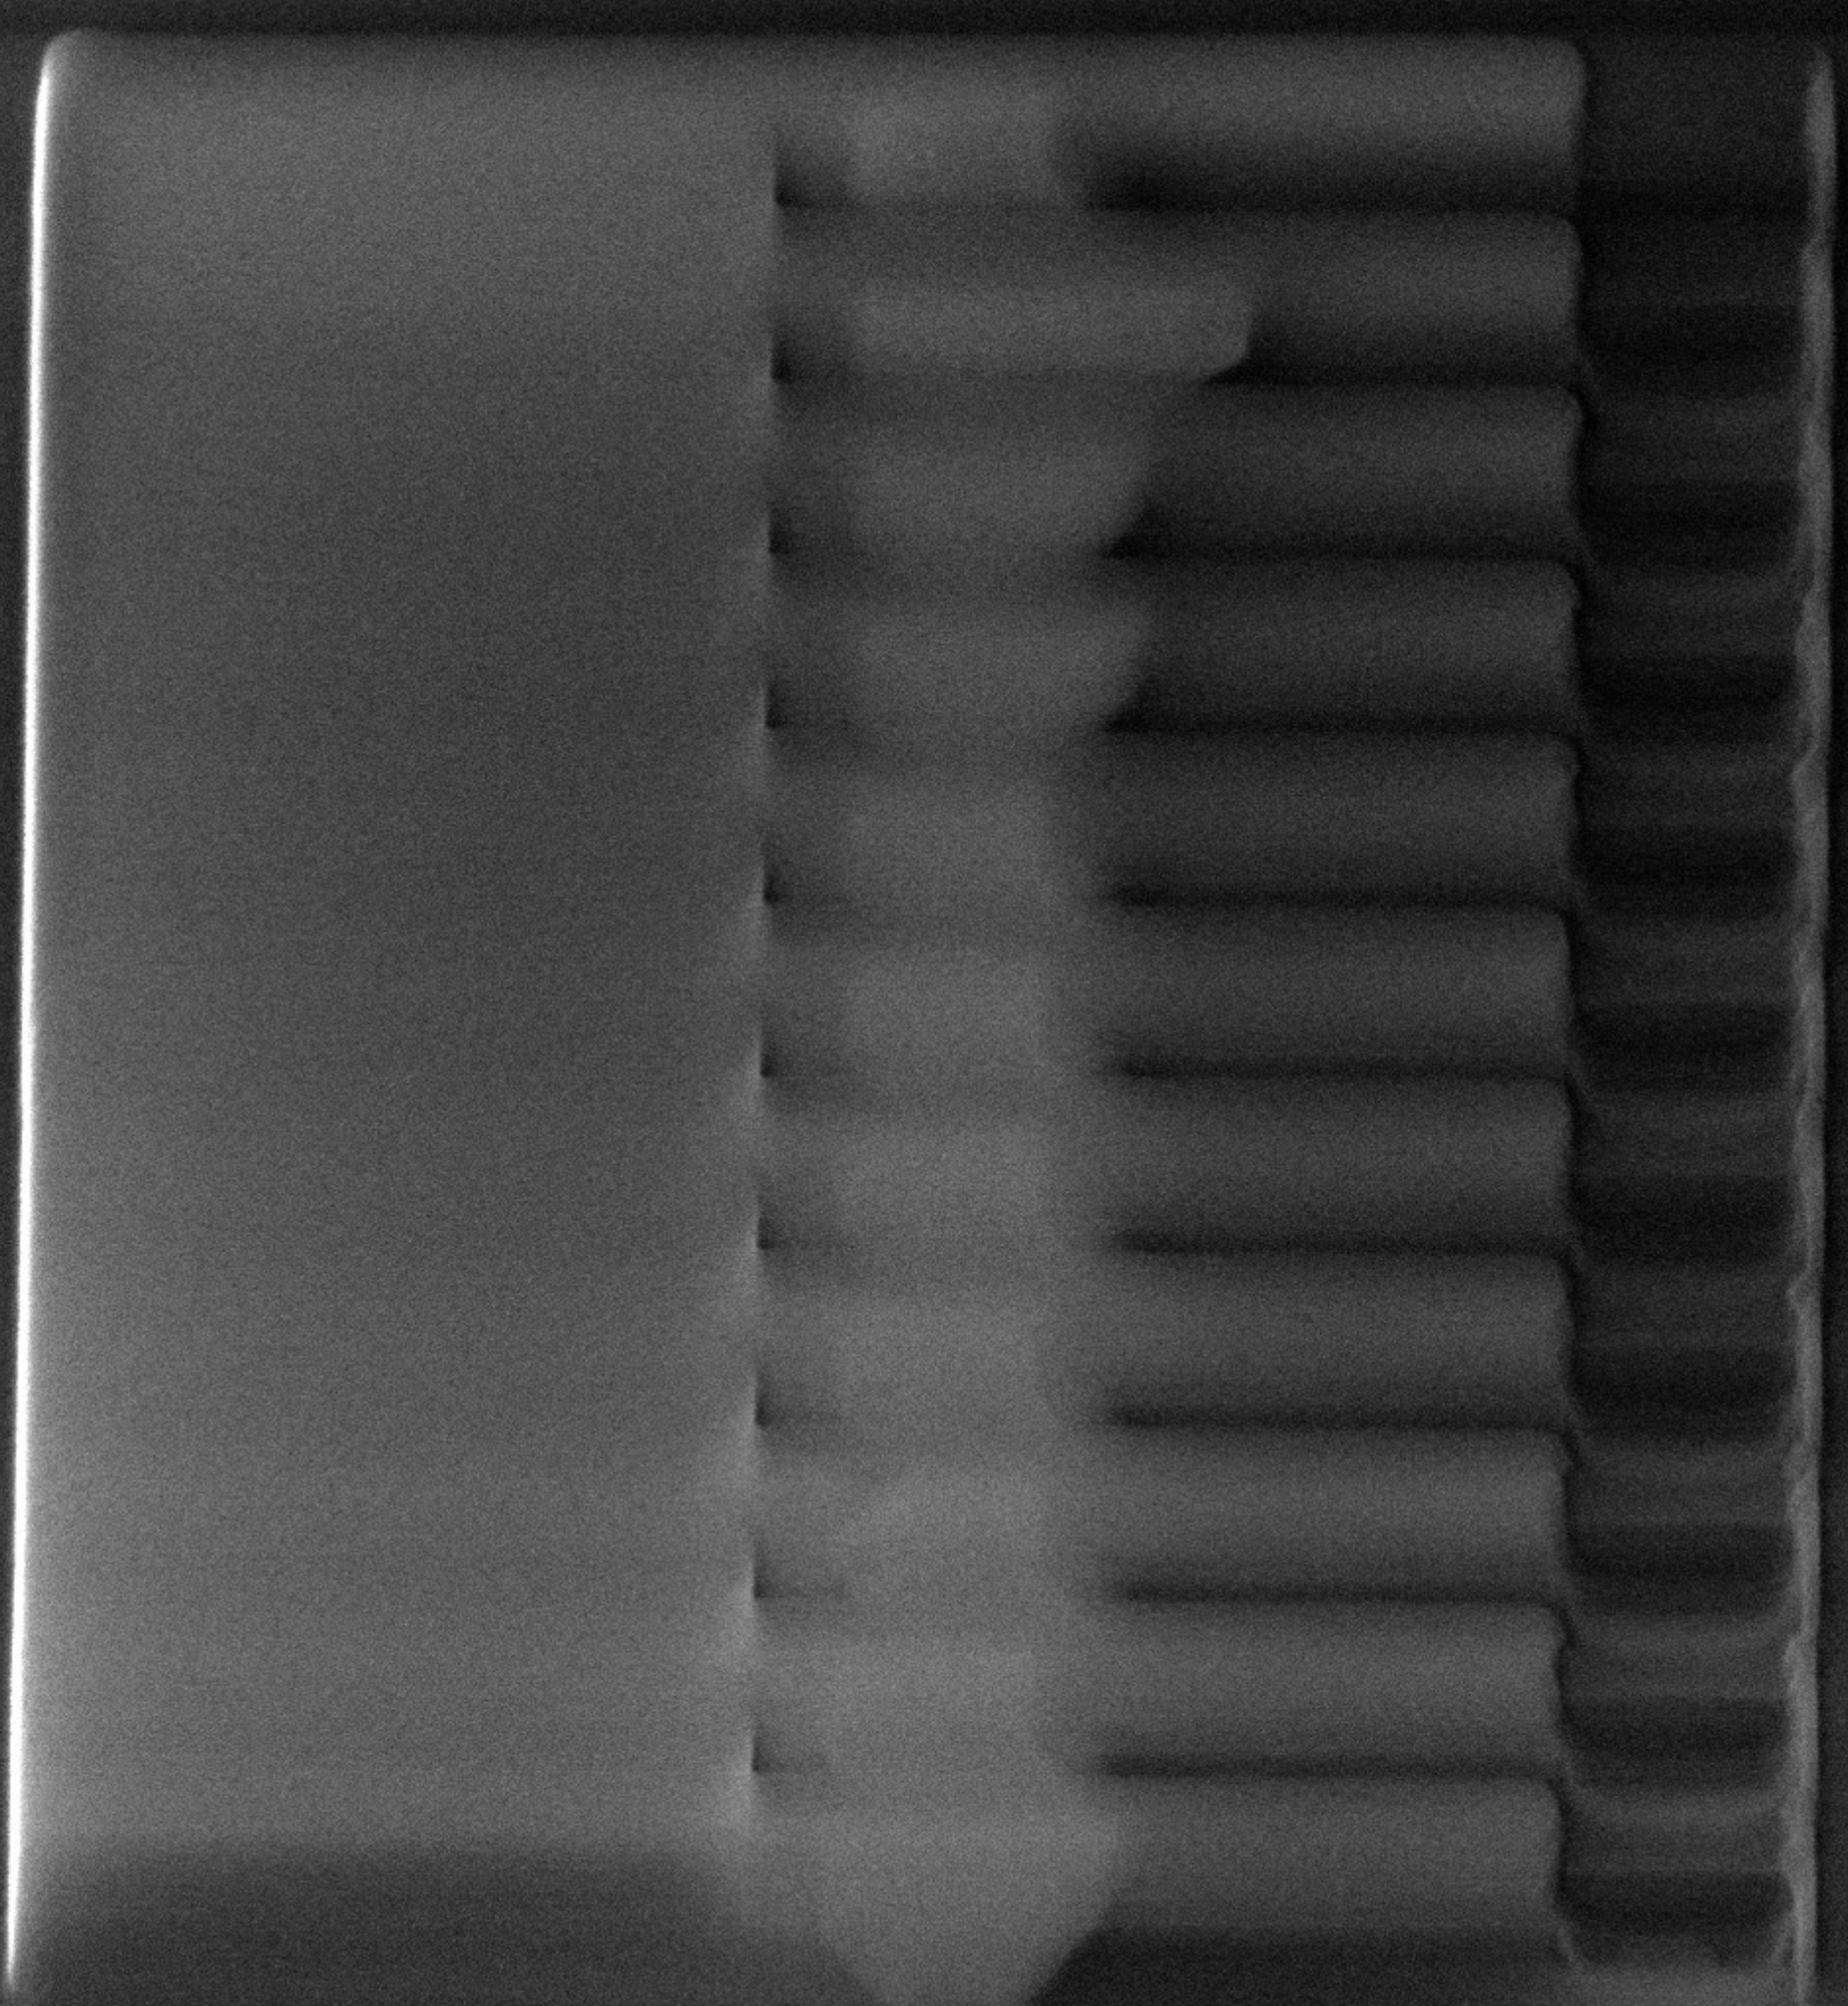
\includegraphics[width=0.6\textwidth]{3_Growth/Comb_Array_001.pdf}};
        \draw [|-|, white, very thick] (-4.6, -4) -- (-1, -4) node [midway, anchor=south] {\qty{1}{\micro\metre}};
        \draw [|-|] (-4.8, -5.5) -- (-0.4, -5.5) node [midway, anchor=north]{\acs{si} backbone and seed};
        \draw [|-|] (-0.4, -5.5) -- (0.9, -5.5) node [midway, anchor=north]{III-V};
        \draw [|-|] (0.9, -5.5) -- (3.2, -5.5) node [midway, anchor=north]{template};
        \draw [|-|] (3.2, -5.5) -- (4.7, -5.5) node [midway, anchor=north]{opening};
    \end{tikzpicture}
    }
    \caption[Growth recipe and \acs{sem_m} image of sample 1.]{Growth of the first sample. \subref{subfig:recipe1} diagram representing the growth recipe for a single-heterointerface III-V wire \cite{Brugnolotto2023}. Each line represents an active flow of precursor into the reactor. The colour of the horizontal lines represents the target material. \subref{subfig:comb_sample1} shows a \acs{sem_m} image of an \num{11}-nanowire array. The \acs{si} seed, III-V segment, empty template, and template opening are visible from left to right.}
    \label{fig:sample1_growth}
\end{figure}

\begin{table}
    \centering
    \caption[V/III molar ratios injected in the reactor during each material deposition step.]{V/III molar ratios injected in the reactor during each material deposition step \cite{Brugnolotto2023_2}.}
    \begin{tabular}{l|c}
        Material & V/III ratio \\ \hline \hline
        InGaAs  & 234\\
        InP     & 29\\ \hline
    \end{tabular}
    \label{tab:sample1_ratios}
\end{table}

The second key factor in determining the shape of the growing crystal is the individual growth rate of each facet. Growth conditions, including temperature, precursor molar flow, III/V ratios, and chemical species, are the key to determining the low-index facet growth rate \cite{Borg2015, Elsner1992}.
\par
After all the fabrication and pre-processing steps, the growth of III-V material occurs in an \acf{mocvd} reactor at \qty{580}{\degreeCelsius}. The recipe used for the first growth experiment is shown in Figure~\ref{subfig:recipe1}. In this image, the flow of a precursor into the reactor is represented by a horizontal line, and the colour of each line indicates the target material.

The objective of this growth run was to study the evolution of growth and evaluate the effects of the growth parameters on the morphology of the two material segments. Two different III-V segments were grown for this sample with the deposition times of \qty{420}{\second} and \qty{240}{\second} for the \acs{ingaas} and \acs{inp} segments, respectively. Table~\ref{tab:sample1_ratios} summarises the V/III molar ratios used. These were chosen according to those used in previous experiments to aid in recognising patterns that could be improved upon during growth without unexpectedly influencing parameters such as nucleation yield and growth rates.

The \acs{sem_m} image in Figure~\ref{subfig:comb_sample1} shows a comb array with \num{11} nanowires after \acs{mocvd} growth. The structure segments are marked: on the right side of the image, the holes through which the precursors entered the templates are visible. The image was captured with the sample fixed on a stage that was tilted \qty{52}{\degree} with respect to the \hkl<0 0 1> direction in the device layer of the \acs{soi} device layer before \acs{fib} cutting. The shape of the end-faced of each nanowire is visible due to the tilt, with most wires terminating with a \hkl{1 1 1}\(_B\) facet. Only one of the wires, the second one from the top, appears to have a different end-facet. The third wire from the bottom presents an interesting (but not unique, as shown in \cite{Scherrer2022}) situation where the growing crystal leaves the seed partially uncovered. Two \hkl{1 1 0} facets form an arrowhead-like shape, indicating the presence of faster growth in the \hkl<1 1 1> direction compared to the \hkl<1 1 0> directions immediately after nucleation.

\subsection{\texorpdfstring{\acs{fib} lamella fabrication}{FIB lamella fabrication}}

\begin{figure}
    \centering
    \subcaptionbox{
        \acs{sem_m} image of an electron transparent lamella \cite{Brugnolotto2023}.
        \label{subfig:FIB_cut}
        }{
        \tikzsetnextfilename{FIB_cut}
        \begin{tikzpicture}
            \node[inner sep=0pt] (image) at (0,0) {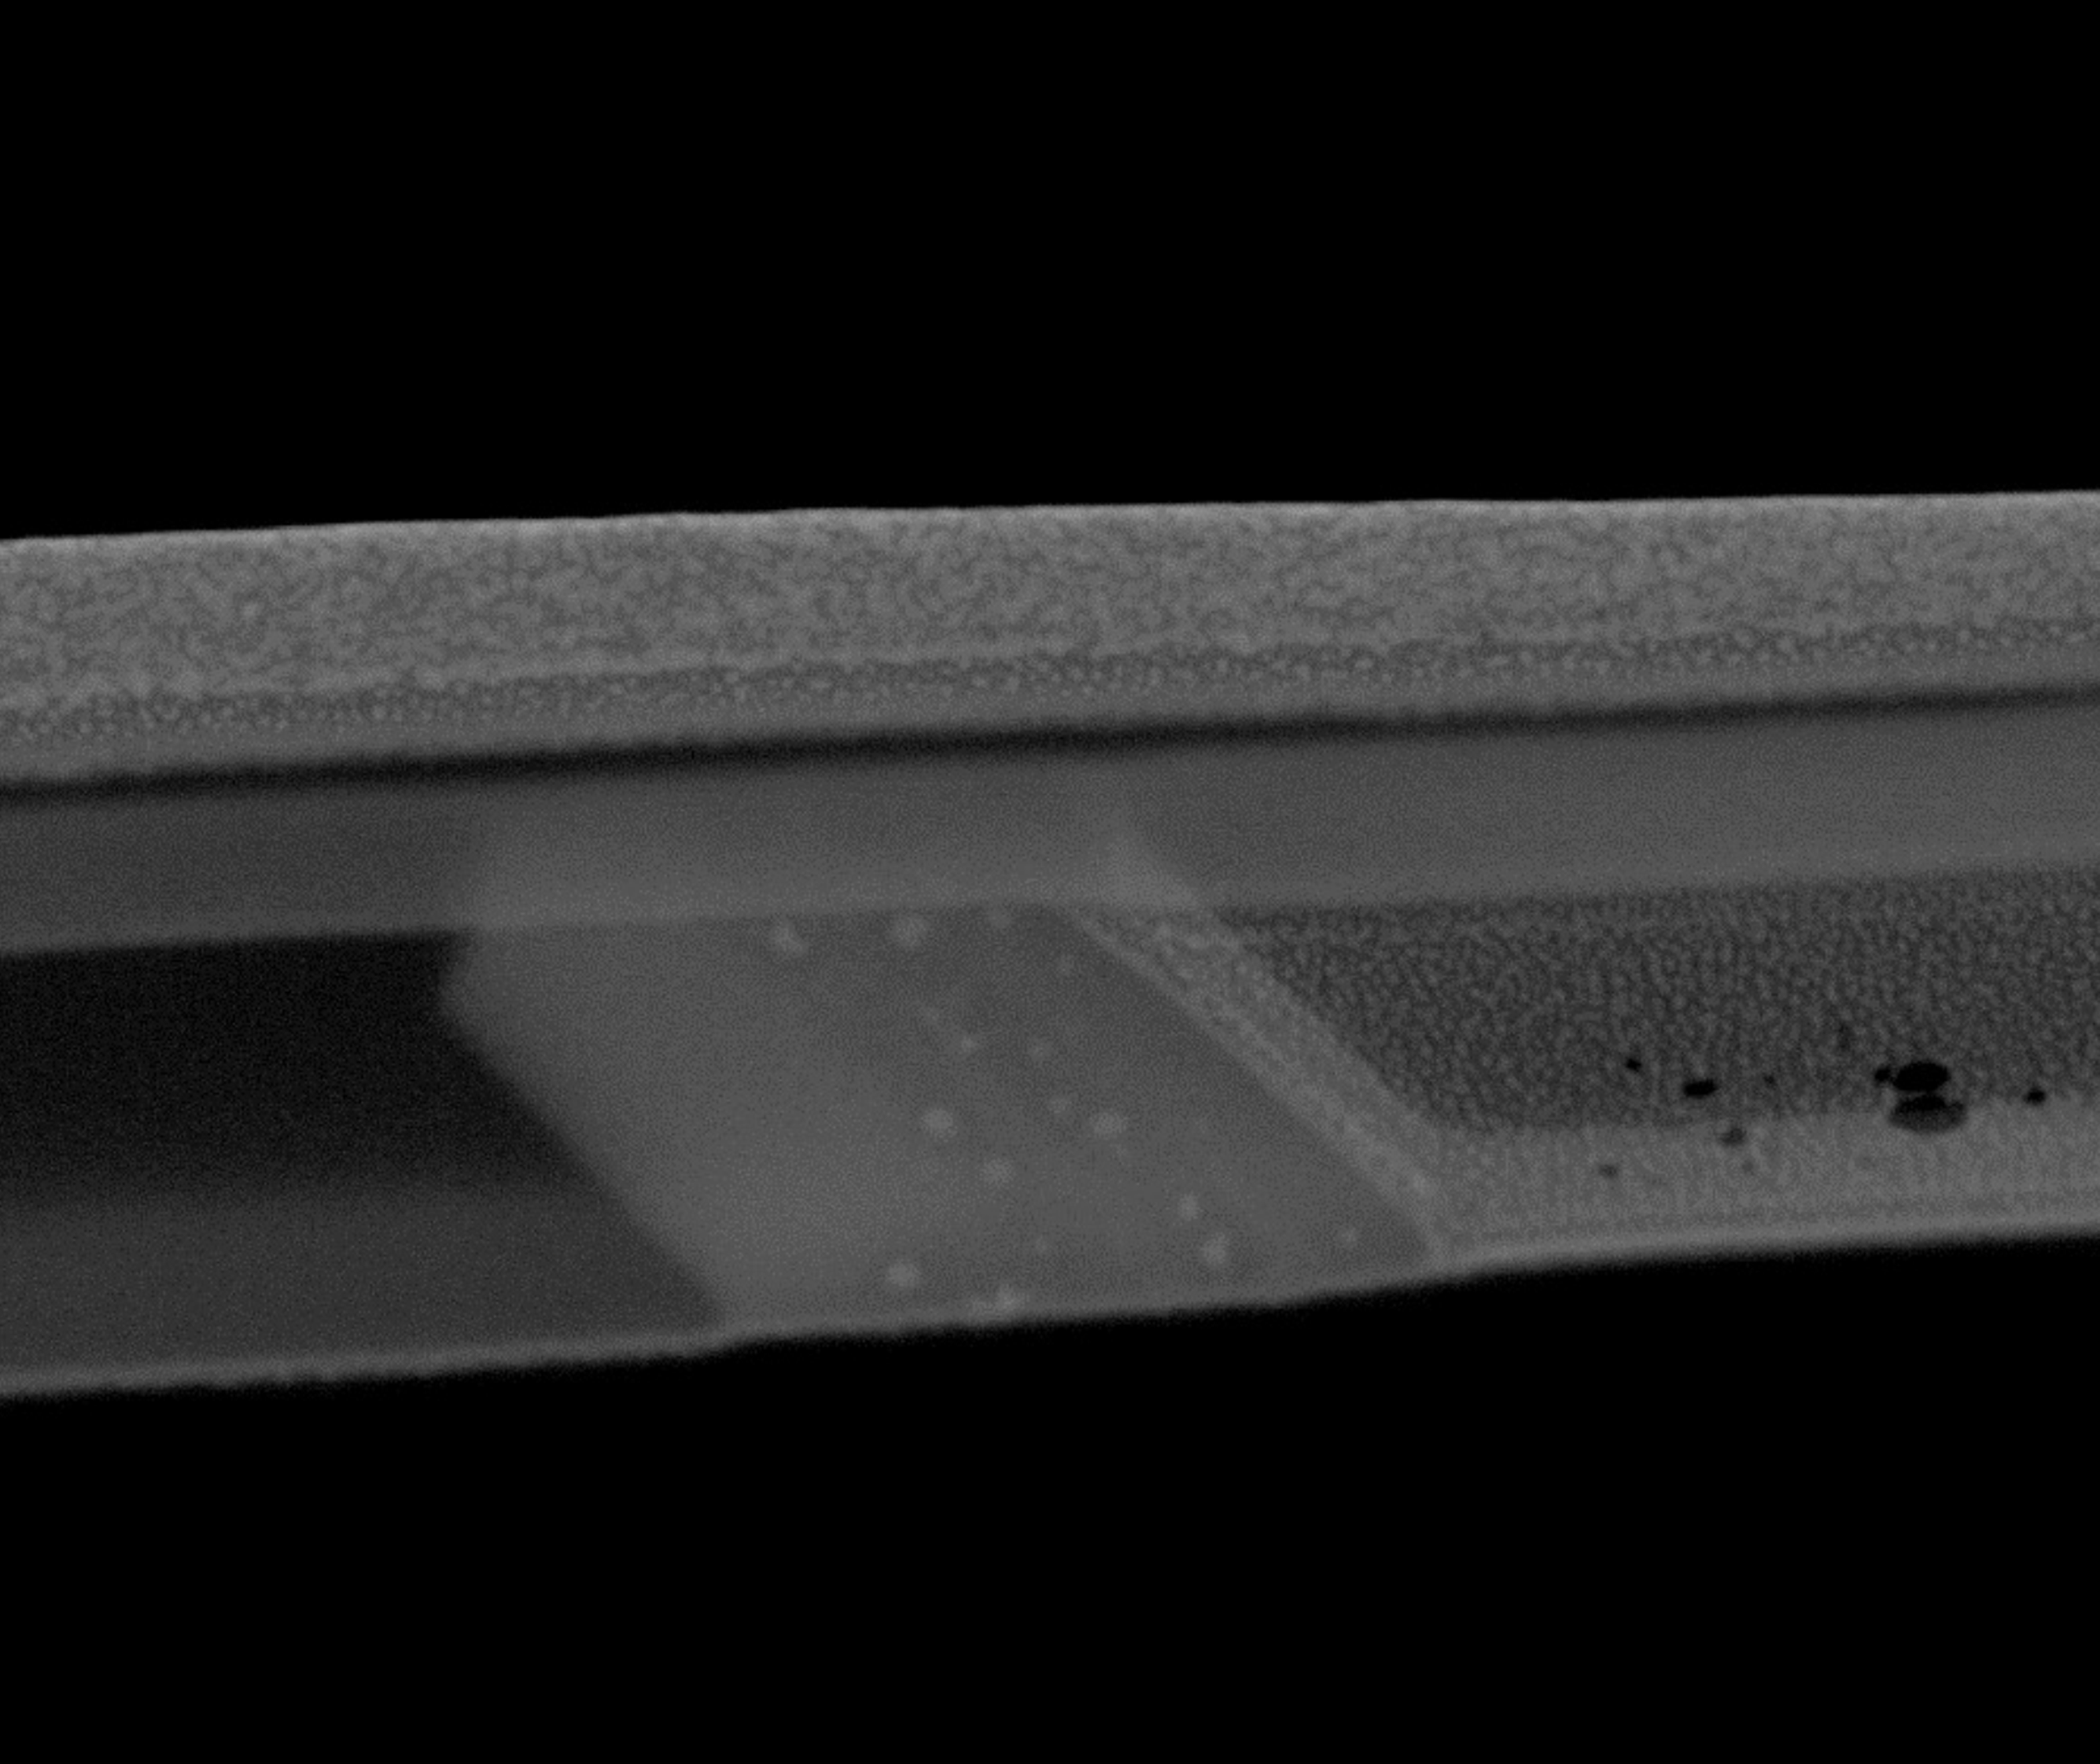
\includegraphics[width=0.48\textwidth]{3_Growth/FIB_Cut.pdf}};
            \node [text=white,] at (-2, -2.5) {\acs{sio2}};
            \node [text=white] at (2, 0.3) {\acs{sio2}};
            \node [text=white] at (0, -0.7) {III-V};
            \node [text=white] at (-2.5, -1) {\acs{si}};
            \node [text=white] at (0, 1) {\ce{Pt}};
            \node [text=white] at (2, -0.5) {Void};
        \end{tikzpicture}
    }
    \subcaptionbox{
        Cutting strategy for a cross section in a \hkl(0 0 1) substrate.
        \label{subfig:FIB_cut_strategy}
        }{
        \tikzsetnextfilename{FIB_cut_strategy}
        \begin{tikzpicture}[isometric]
            \path [fill=red!50!, fill opacity=0.3] (-0.5, -0.3, 0.5) -- (-0.5, 1.5, 0.5) -- (5.5, 1.5, 0.5) -- (5.5, -0.3, 0.5) -- cycle;
            \path [fill=red!50!, fill opacity=0.3] (-0.5, -0.3, 1.5) -- (-0.5, 1.5, 1.5) -- (5.5, 1.5, 1.5) -- (5.5, -0.3, 1.5) -- cycle;
            
            \draw (0, 0, 0) -- (0, 0, 2) -- (0, 1, 2) -- (0, 1, 0) -- cycle;
            \draw (0, 0, 0) -- (3, 0, 0) -- (3, 1, 0) -- (0, 1, 0);
            \draw (0, 0, 2) -- (3, 0, 2) -- (3, 1, 2) -- (0, 1, 2);
            \draw (3, 0, 0) -- (3, 0, 2);
            \draw (3, 1, 0) -- (3, 1, 2);
            
            \draw (-0.2, 0, -0.2) -- (-0.2, 0, 2.2) -- (-0.2, 1.2, 2.2) -- (-0.2, 1.2, -0.2) -- cycle;
            \draw (-0.2, 0, -0.2) -- (5, 0, -0.2) -- (5, 1.2, -0.2) -- (-0.2, 1.2, -0.2);
            \draw (-0.2, 0, 2.2) -- (5, 0, 2.2) -- (5, 1.2, 2.2) -- (-0.2, 1.2, 2.2);
            \draw (5, 0, -0.2) -- (5, 0, 2.2);
            \draw (5, 1.2, -0.2) -- (5, 1.2, 2.2);
            
            \draw [red, dashed] (-0.2, 0, 0.5) -- (5, 0, 0.5) -- (5, 1.2, 0.5) -- (-0.2, 1.2, 0.5) -- cycle;
            \draw [red, dashed] (-0.2, 0, 1.5) -- (5, 0, 1.5) -- (5, 1.2, 1.5) -- (-0.2, 1.2, 1.5) -- cycle;

            \draw [-stealth] (5, 5, 1) -- (6, 5, 1) node[anchor=west]{\hkl<1 1 0>};
            \draw [-stealth] (5, 5, 1) -- (5, 6, 1) node[anchor=south]{\hkl<0 0 1>};
            \draw [-stealth] (5, 5, 1) -- (5, 5, 2) node[anchor=east]{\hkl<-1 1 0>};
        \end{tikzpicture}
    }
    \caption[\acs{fib} cut strategy and result for samples grown on \hkl(0 0 1) \acs{soi}.]{\acs{fib} cut of a lamella from a \hkl<0 0 1> \acs{soi} wafer. \subref{subfig:FIB_cut} shows the \acs{sem_m} image of a thinned electron-trasparent lamella. The various materials are marked, and the structure is discernible. \subref{subfig:FIB_cut_strategy} shows how the cut is made within the context of the crystalline and growth directions. The red-shaded planes show that we select the cut to expose the sides of the wire in correspondence to a \hkl{-1 1 0} plane if we label the template axis as a \hkl<1 1 0> direction.}
    \label{fig:001_FIB}
\end{figure}

A high-resolution analytical method is needed to analyse the type of structures shown in Figure~\ref{subfig:enterprise_design}. Indeed, their small size means that, for example, X-ray analysis with laboratory-sized tools is unfeasible. Instead, microscopy techniques are particularly powerful, with high-end \acf{tem_m} or \acf{stem_m} able to resolve features up to atomic resolution and provide important structural information. However, an electron-transparent lamella is required to analyse material layers and investigate the morphology of internal heterointerfaces. \Acf{fib} tools can create these <\qty{100}{\nano\metre} thin semiconductor cross sections. In this study, an FEI Helios NanoLab 450S was used.
\par
Figure~\ref{subfig:FIB_cut} shows how one lamella looks once \acs{fib} cutting is complete. This image is perfect for showcasing the various material portions of the sample while retaining a three-dimensional view, which is lost in the later \acs{stem_m} analysis. The \acl{si} seed is visible on the left, followed by the III-V material layer, which appears brighter in the centre of the image. On the exposed surface of this layer, two areas can be characterised and distinguished by the presence of small \acl{in} droplets (on the right) and their absence (on the left). These \acl{in} droplets are commonly formed during the ion milling of \acl{inp} at the \acs{fib} tool. On the right side, the empty template is filled with a \acl{pt} lace-like structure formed when the protection layer was deposited before the lamella was cut from the chip. The upper and lower interfaces of the template are visible in this image, appearing as two ribbons or bands above and below the \acl{si} / III-V / void structure. In particular, the upper interface is the most visible; they can be easily spotted by looking at the \acl{si} region. What remains of the \acl{pt} protective layer is also noticeable as a bright region at the very top of the structure.
\par
The objective of the cut strategy shown in Figure~\ref{subfig:FIB_cut_strategy} is two-fold. The first aim is to provide a lamella that showcases both the seed and end facets to evaluate the evolution of the growth front, and the second is to have access to a low-index facet that can provide structural information on the quality of the lattice. For the zincblende phase, the second criterion is satisfied by \hkl{1 1 0} facets \cite{Dasilva2017}. In a \hkl{0 0 1} \acs{soi} there is an in-plane \hkl[-1 1 0] direction perpendicular to the \hkl[1 1 0] direction along which the template is orientated. This means that a simple cross-section along the wire allows access to the maximum information about the nanowire.

\subsection{\texorpdfstring{\acs{stem_m} analysis}{STEM analysis}}

\begin{figure}
    \centering
    \subcaptionbox{
        \acs{bf}-\acs{stem_m} overview of a III-V nanowire cross-section.
        \label{subfig:sample1_cross-sec}
        }{
        \tikzsetnextfilename{sample1_cross-sec}
        \begin{tikzpicture}
            \node[inner sep=0pt] (image) at (0,0) {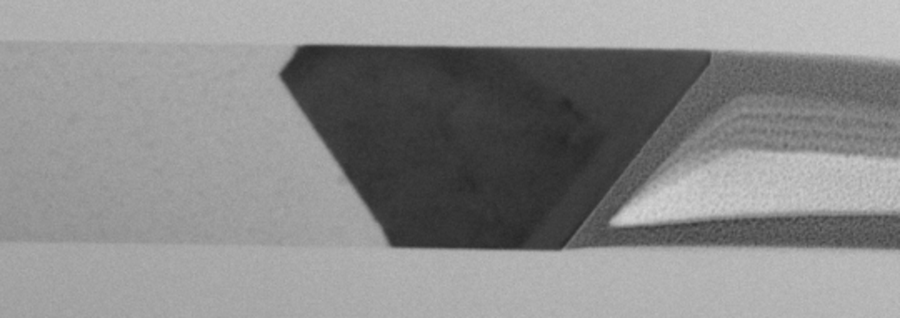
\includegraphics[width=\textwidth]{3_Growth/Sample1_Overview.pdf}};
            \draw [red] (1.25, -1.63) -- (2.9, 0.5); %1.65, 2.13
            \draw [red, dashed] (0.95, 1.93) -- (2.9, 0.5) -- (3.35, 1.1) -- (2.2, 1.93);
            \draw [orange] (2, -1.63) -- (4.65, 1.7) -- (4.7, 1.93);
            \draw [yellow] (-3.3, 1.2) rectangle (-2.7, 1.8);
            \draw [|-|, very thick] (-7.4, -2.5) -- (-4, -2.5) node [midway, anchor=south] {\qty{1}{\micro\metre}};
            \node [text=white] at (5.5, 1.5) {\ce{Pt}};
            \node at (-2, -2) {\acs{sio2}};
            \node at (2, 2.4) {\acs{sio2}};
            \node [text=white] at (0, -0.7) {\acs{ingaas}};
            \node [text=white] at (3.5, 1.5) {\acs{inp}};
            \node at (-2.5, -0.7) {\acs{si}};
            \node at (5, -0.5) {Void};
        \end{tikzpicture}
    }
    \subcaptionbox{
        \acs{eds} map: red-\acs{in}, green-\acs{si}, blue-\acs{ga}.
        \label{subfig:s1_III_EDS}
    }{
        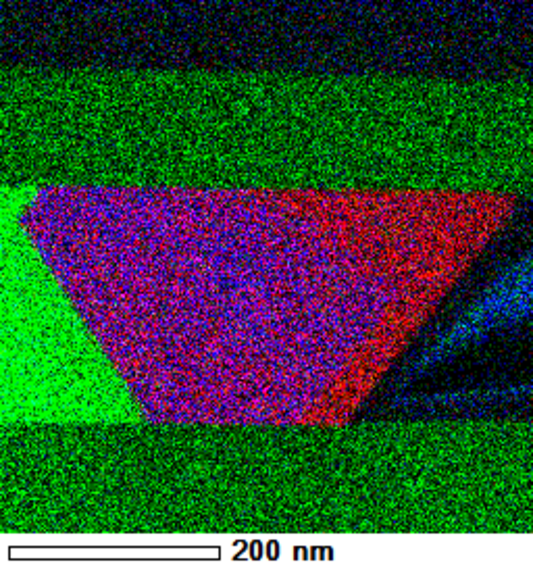
\includegraphics[width=0.45\textwidth]{3_Growth/s1_III_EDS.pdf}
    }
    \subcaptionbox{
        \acs{eds} map: red-\acs{as}, green-\acs{p}, blue-\acs{in}.
        \label{subfig:s1_V_EDS}
    }{
        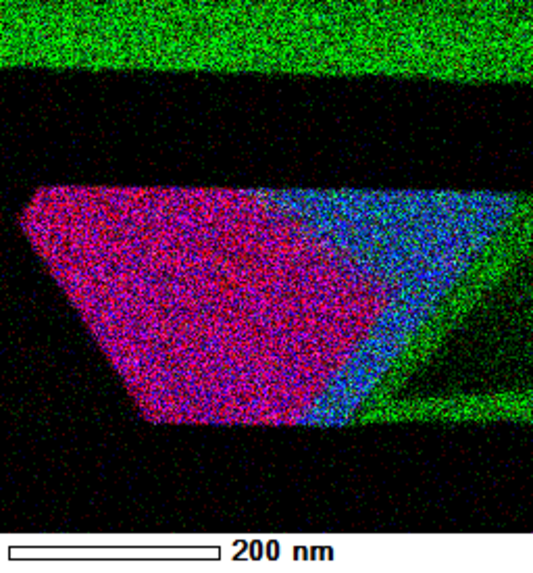
\includegraphics[width=0.45\textwidth]{3_Growth/s1_V_EDS.pdf}
    }
    \subcaptionbox{
        \acs{bf}-\acs{stem_m} detail of the \acs{si}/\acs{ingaas} interface.
        \label{subfig:si-ingaas_s1}
        }{
        \tikzsetnextfilename{si-ingaas_s1}
        \begin{tikzpicture}
            \node[inner sep=0pt] (image) at (0,0) {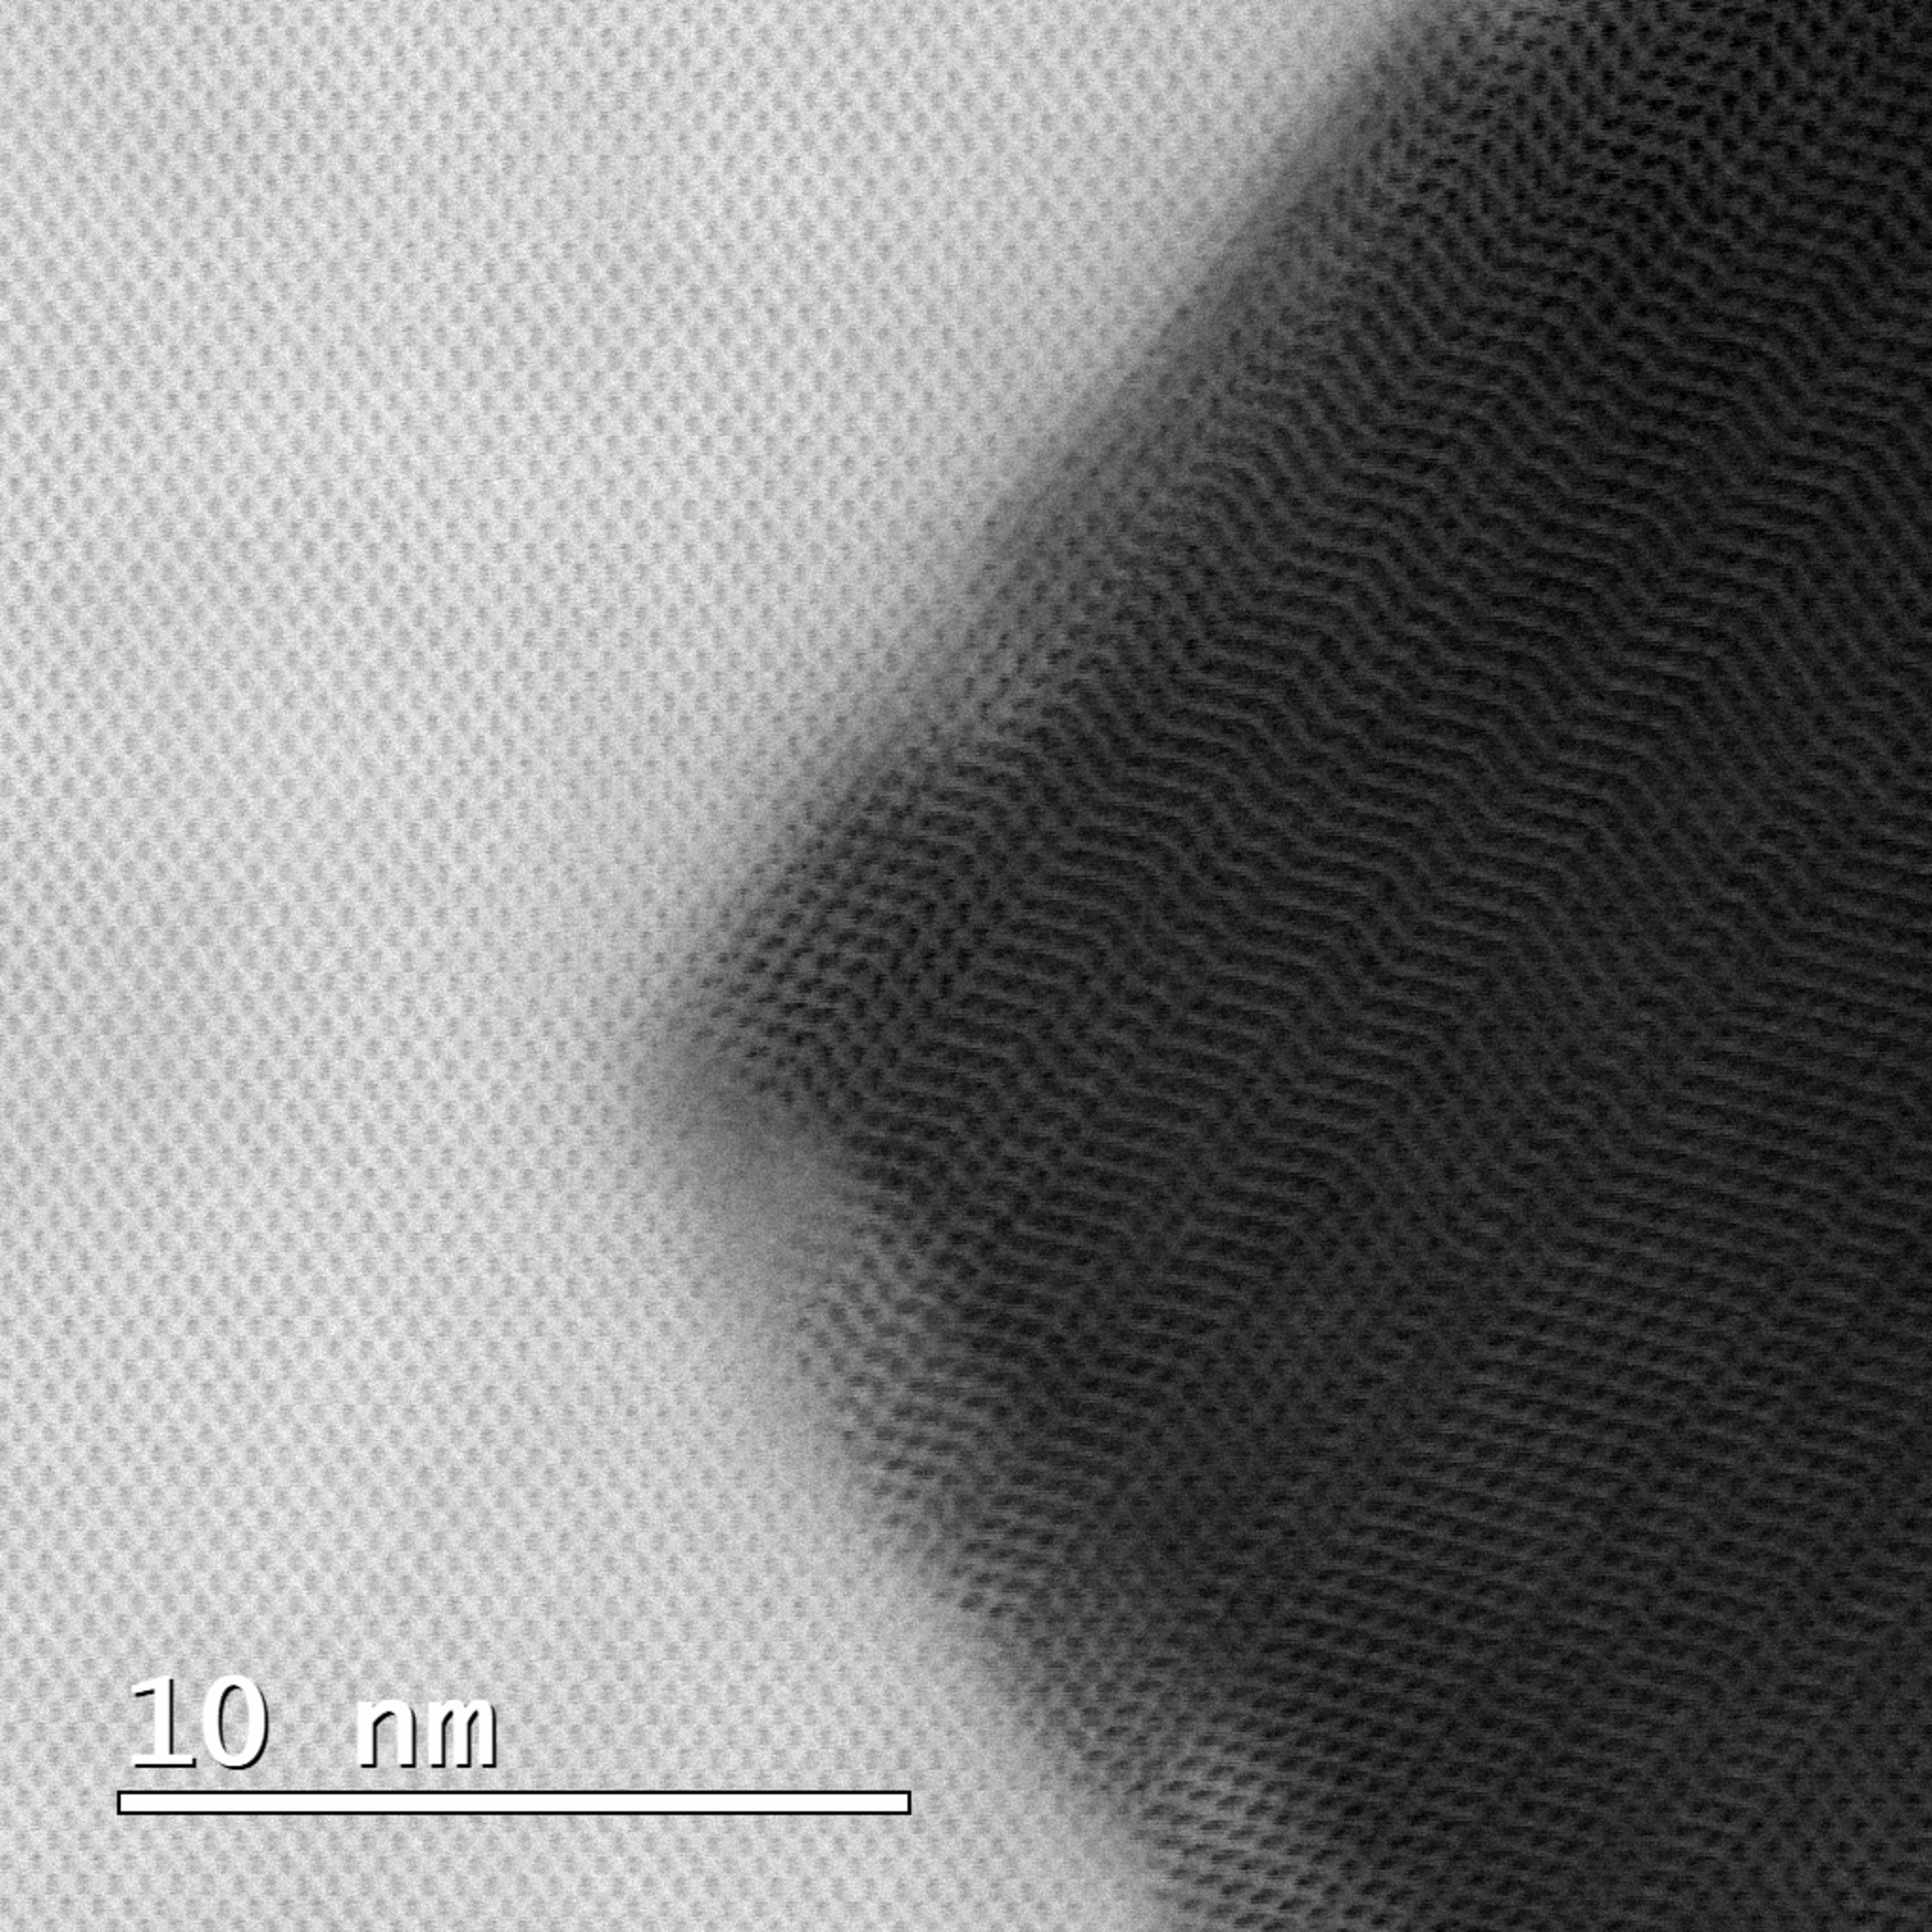
\includegraphics[width=0.45\textwidth]{3_Growth/Si_interface_sample1.pdf}};
            \node [white] at (2, -1) {\acs{ingaas}};
            \node at (-3, 3) {\acs{si}};
        \end{tikzpicture}
    }
    \caption{Overview, composition analysis, and detail of the seed/\acs{ingaas} interface. in sample 1.}
    \label{fig:sample1}
\end{figure}

The bottom-most wire of the array in Figure~\ref{subfig:comb_sample1} was chosen for investigation. Once the \acs{fib} cut was complete, the resulting lamella was cleaned in an \acl{o} plasma for \qty{30}{s} before being loaded in a JEOL ARM 200F \acl{stem_i}. Figure~\ref{subfig:sample1_cross-sec} shows an overview image of the lamella imaged with the \acf{bf} detector of the \acs{stem_m}. The difference in atomic number gives contrast to the image through what is known as Z-contrast: material composed of heavier atoms will appear darker in a \acs{bf} image, and vice versa in an \acf{adf} or \acf{haadf} image. Therefore, the darkest area of the sample is the \acs{ingaas} layer, as its III and V components have a high atomic number. \acs{inp} appears a bit brighter given that the V group element, \acl{p}, is light. The \acl{si} and \acs{sio2} layers are very bright in comparison, as the small \acl{si} and \acl{o} atoms allow the transmission of a higher portion of the beam. The contrast of the \acs{fib}-deposited \acl{pt} is modulated by its thickness and lower density. The red and orange lines in this figure highlight the two segments. The red line shows the limit of the \acs{ingaas} segment, with the top dashed lines signifying the presence of a facet tilted from the observation direction. The orange lines show the limit of the \acs{inp} segment. The Z-contrast's compositional clues are confirmed by spectroscopic analysis in Figure~\ref{subfig:s1_III_EDS} and Figure~\ref{subfig:s1_V_EDS}. 
\par
\paragraph{Spectroscopic analysis}Figure~\ref{subfig:s1_III_EDS} shows a low-resolution compositional map created with the \acf{eds} data from the sample in Figure~\ref{subfig:sample1_cross-sec}. The map is colour-coded with each colour representing the intensity of an element-specific spectroscopic line processed to consider the cross-section of each transition. This creates the compositional map. Areas that appear more red have a higher \acl{in} concentration, those that appear green have a high \acl{si} content, and those with a blue tinge contain \acl{ga}. The brightness of its colour carries information regarding the amount of each element present in each region. For example, the \acl{si} signal is stronger in the seed area on the left of the image and fainter in the top and bottom \acs{sio2} template and buried oxide areas. \Acl{in} signal is present throughout the III-V area, as expected given the two \acs{ingaas} and \acs{inp} layers. The \acl{ga} signal is mostly confined to the \acs{ingaas} layer, but a small blue tint can be noticed in correspondence with the outer \acl{pt} region inside the template on the right centre of the map. This is due to the \acs{fib} processing causing redeposition. Indeed, some green dots from the redeposited \acl{si} can also be spotted in that map area. The absence of \acl{in} signal could be attributed to the tendency of this material to form droplets, as seen in Figure~\ref{subfig:FIB_cut}.
\par
Another \acs{eds} map of the lamella in Figure~\ref{subfig:sample1_cross-sec} investigating the distribution of V group elements is shown in Figure~\ref{subfig:s1_V_EDS}. Here, \acl{as} appears in red, \acl{p} in green, and \acl{in} in blue. The \acl{in} signal allows for the determination of the III-V area, as it is present in both \acs{inp} and \acs{ingaas}. The \acl{as} signal defines the \acs{ingaas} area, and the green dots revealing the presence of \acl{p} are also present in the remaining \acs{in}-rich area. What appears, upon first examination, to be further \acl{p} high concentration in the \acs{fib}-deposited \acl{pt} is also noticeable. However, this signal can be better explained by examining the energy at which the \acl{p} K\(_\alpha\) line is located. Indeed, the \acs{p} K\(_\alpha\) line at \qty{2.013}{\kilo\eV} is very close to the \acl{pt} M line, which falls at \qty{2.048}{\kilo\eV}. These two energies are too close for the two peaks to be distinguished when peak width and spectral resolution are taken into account, generating the "fake" \acl{p} signal in the platinum layers.
\par
\paragraph{Heterointerfaces}This sample presents three interfaces of interest: \acl{si}/\acs{ingaas}, \acs{ingaas}/\acs{inp}, and \acs{inp}/empty template. Figure~\ref{subfig:si-ingaas_s1} shows the first interface at the "V" corner marked with a yellow square in Figure~\ref{subfig:sample1_cross-sec}. Here, the epitaxial relation between the two lattices is visible. The surface of the \acl{si} seed has some roughness, as made evident by the varying intensity of the \acs{ingaas} image in the first \num{6} III-\acs{as} layers. \Acl{rtp}s parallel to the upper \hkl{1 1 1} \acl{si} facet are also visible in this high-resolution image. The shape of this first interface is defined by the \acs{tmah} etch-back before growth, but the next interface, between \acs{ingaas} and \acs{inp}, is determined by the growth parameters in the reactor. Its shape is consistent with that seen in \cite{Scherrer2022, Borg2017, Borg2015}, with a lower \hkl{1 1 1} facet (marked with a red full line) and an upper \hkl{1 1 0} facet (traced on its expected position in a dashed red line), which is likely one of two. Interestingly, this \hkl{1 1 0} facet disappears almost completely after the growth of the \acs{inp} layer, leaving only a long \hkl{1 1 1} facet and a smaller \hkl{1 1 0} facet at the top. The \hkl{1 1 1} facet is parallel to the \acs{rtp}s and, therefore, the upper \acl{si} interface. Looking back at the array of nanowires in Figure~\ref{subfig:comb_sample1}, the selection of which starting \hkl{1 1 1} facet the end-facet is parallel to appears to be random.
\par

\begin{table}
    \centering
    \caption{Growth rates for the first grown sample.}
    \begin{tabular}{l|c c c}
                    & \multicolumn{3}{c}{Growth rates (\nmmin)}                                                                                                   \\
       Layer        & \hkl<1 1 1>                                   & Longest distance                              & Shortest distance                           \\ \hline \hline
       \acs{ingaas} & \num[separate-uncertainty=true]{46.5 (0.1)}   & \num[separate-uncertainty=true]{51.8 (0.2)}   & \num[separate-uncertainty=true]{20.0 (0.2)} \\
       \acs{inp}    & \num[separate-uncertainty=true]{9.1 (0.2)}    & \num[separate-uncertainty=true]{57.2 (0.8)}   & \num[separate-uncertainty=true]{9.1 (0.2)}  \\ \hline
    \end{tabular}
    \label{tab:sample1_growth_rates}
\end{table}

\paragraph{Growth rates} An attempt to estimate the growth rate of \acs{ingaas} and \acs{inp} can be made. However, multiple reference points can be taken to measure between them because the shape of the seed and end facet are complex. Three different measurements were made for each layer: \hkl<1 1 1>, longest distance, and shortest distance; the first category means that the distance between the two parallel \hkl{1 1 1} facets is measured to calculate the growth rate. For \acs{inp}, the \hkl<1 1 1> and shortest distance growth rates coincide. For the \hkl<1 1 1> growth rates, the difference between \acs{ingaas} and \acs{inp} is particularly high, and so is the difference between the longer distance and the \hkl<1 1 1> growth rates of \acs{inp}. This suggests that the \acs{inp} growth rate in the \hkl<1 1 0> direction is higher than that in the \hkl<1 1 1> direction.

\section{Introduction of thin material layers}

Regarding growth dynamics, the main finding from the sample in Figure~\ref{fig:sample1} is the trend towards stabilisation of the \hkl{1 1 1} growth front during \acs{inp} growth. However, many optoelectronic devices rely on harnessing the properties of quantum confinement structures, and there is no one thin enough layer in sample 1 to constitute one. Therefore, an effort was made to introduce short material deposition segments in the growth recipe and study how they modified and manifested in the final nanowire morphology and composition.

\subsection{Growth recipe for the introduction of short material segments.}

\begin{figure}
    \centering
    \subcaptionbox{
    Growth recipe for sample 2 \cite{Brugnolotto2023}.
    \label{subfig:recipe2}
    }{
        \tikzsetnextfilename{recipe2}
    \begin{tikzpicture}
    \begin{scope}
    % lines
        \node [label={[label distance=0]180:\acs{in}}] at (0, 0) {};
        \draw [cb1_orange, ultra thick] (0, 0) -- (4.2, 0);
        \draw [cb1_dark_blue, ultra thick] (4.2, 0) -- (6.6, 0);
        \draw [cb1_dark_blue, ultra thick] (6.6, 0) -- (7.35, 0);
        \draw [cb1_orange, ultra thick] (7.35, 0) -- (8.1, 0);
        
        \node [label={[label distance=0]180:\acs{ga}}] at (0, -0.5) {};
        \draw [cb1_orange, ultra thick] (0, -0.5) -- (4.2, -0.5cm);
        \draw [cb1_orange, ultra thick] (7.35, -0.5) -- (8.1, -0.5);
        
        \node [label={[label distance=0]180:\acs{as}}] at (0, -1) {};
        \draw [cb1_orange, ultra thick] (0, -1) -- (4.2, -1);
        \draw [cb1_orange, ultra thick] (7.35, -1) -- (8.1, -1);
        
        \node [label={[label distance=0]180:\acs{p}}] at (0, -1.5) {};
        \draw [cb1_dark_blue, ultra thick] (4.2, -1.5) -- (6.6, -1.5);
        \draw [cb1_dark_blue, ultra thick] (6.6, -1.5) -- (7.35, -1.5);
        
    % labels and markers for the timescale
        \node [label={[label distance=0]180:Time (\second)}] at (0, -2) {};
        \draw [-stealth] (0, -2) -- (8.4, -2);
        \draw [] (0, 0.2) -- (0, -2.2) node[anchor = north] {\num{0}};
        \draw [] (4.2, 0.2) -- (4.2, -2.2) node[anchor = north] {\num{420}};
        \draw [] (6.6, 0.4) -- (6.6, -2.2) node[anchor = north] {\num{660}};
        \draw [] (7.35, 0.2) -- (7.35, -2.2) node[anchor = north] {\num{735}};
        \draw [] (8.1, 0.4) -- (8.1, -2.2) node[anchor = north] {\num{810}};
        \draw [stealth - stealth] (6.6, 0.3) -- (8.1, 0.3) node[midway, anchor=south] {Loop};
    \end{scope}
    \begin{scope} [shift={(9.3cm, -0.5)}]
        \draw [cb1_orange, ultra thick] (0, 0) -- (0.5, 0) node[anchor = west, text=black] {\acs{ingaas}};
        \draw [cb1_dark_blue, ultra thick] (0, -0.5) -- (0.5, -0.5) node[anchor = west, text = black] {\acs{inp}};
        \draw (-0.5, 0.5) -- (2.5, 0.5) -- (2.5, -1.15) -- node[midway, fill = white] {Legend} (-0.5, -1.15) -- cycle;
    \end{scope}
    \end{tikzpicture}
    }
    \subcaptionbox{
        \acs{sem_m} image of the lamella for sample 2.
        \label{subfig:FIB_cut_2}
        }{
        \tikzsetnextfilename{FIB_cut_2}
        \begin{tikzpicture}
            \node[inner sep=0pt] (image) at (0,0) {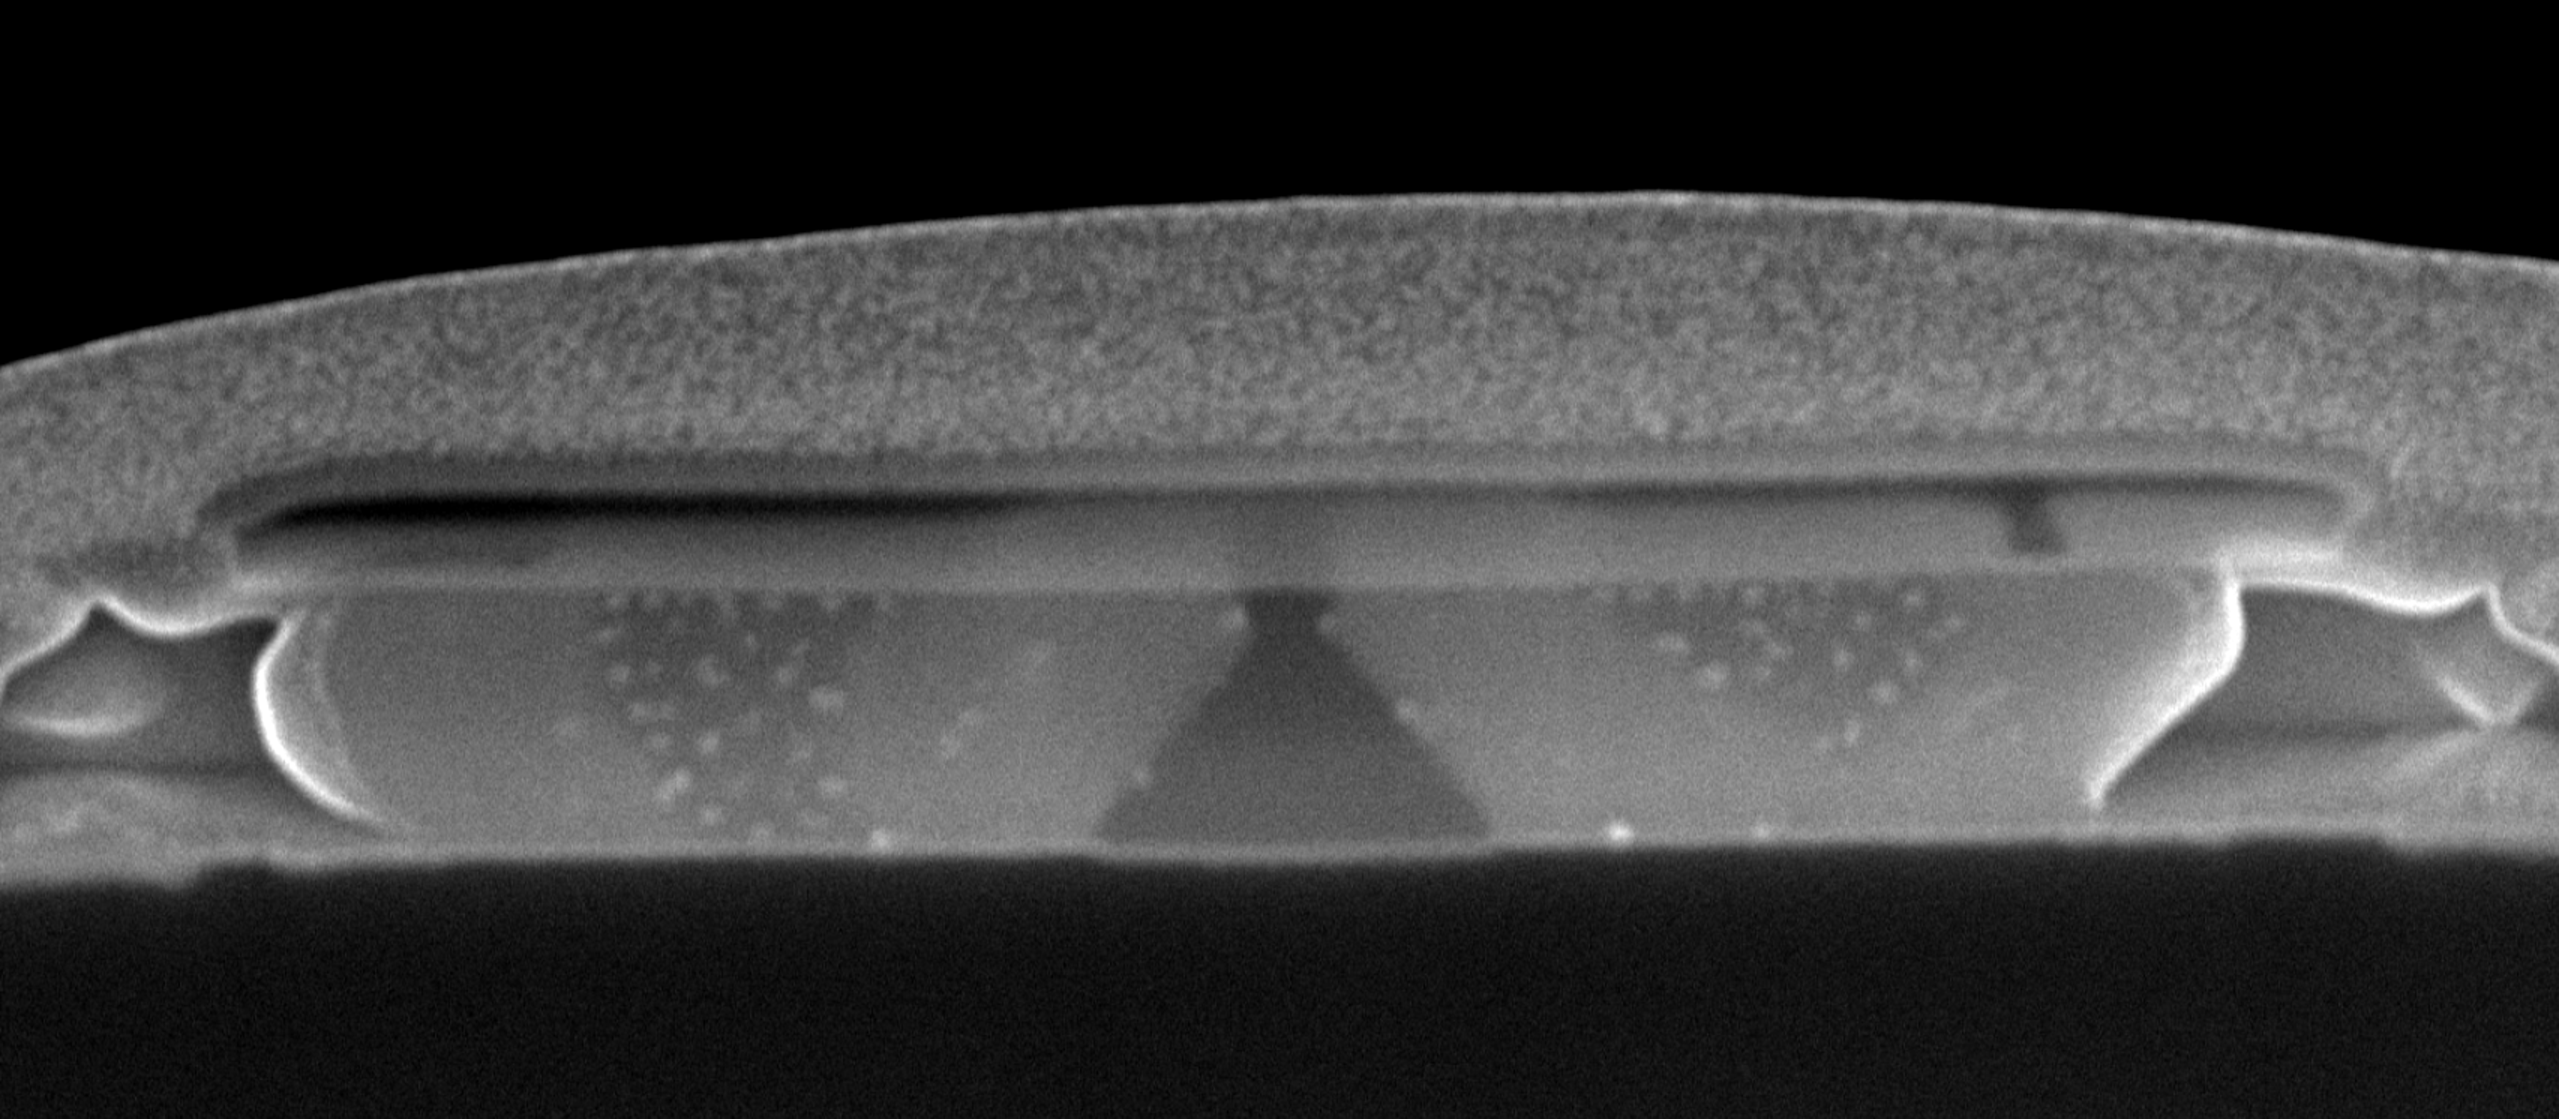
\includegraphics[width = \textwidth]{3_Growth/Sample2_FIB.pdf}};
            \node [text=white,] at (0, -2.5) {\acs{sio2}};
            \node [text=white] at (0, 0.2) {\acs{sio2}};
            \node [text=white] at (-2, -0.7) {III-V};
            \node [text=white] at (2, -0.7) {III-V};
            \node [text=white] at (0, -1.3) {\acs{si}};
            \node [text=white] at (0, 1.5) {\ce{Pt}};
            \node [text=white] at (7, -1) {Void};
            \node [text=white] at (-7, -1) {Void};
            \draw [white, |-|, very thick] (-7.2, 2.8) -- (-3, 2.8) node [midway, anchor=south] {\qty{500}{\nano\metre}};
        \end{tikzpicture}
    }
    \caption[Growth recipe and \acs{sem_m}-\acs{fib} image of a cross-section of a wire from sample 2]{Growth of the second sample. \subref{subfig:recipe1} Is the diagram representing the modified growth recipe introducing the looped segment for thin layer deposition \cite{Brugnolotto2023}. Each line represents an active flow of precursor into the reactor. The colour of the horizontal lines represents the target material. \subref{subfig:FIB_cut_2} \acs{sem_m} image of the lamella during \acs{fib} thinning. The various material regions are labelled.}
    \label{fig:sample2_growth}
\end{figure}

A further looped deposition segment was introduced at the end of the recipe in Figure~\ref{subfig:recipe1} to study the growth of thin structures in the template. The resulting recipe is illustrated in Figure~\ref{subfig:recipe2}. The looped segment, executed twice without interruption, contains an \acs{inp} and an \acs{ingaas} deposition step. The two short deposition steps are \qty{75}{s} long. The growth temperature was kept constant at \qty{580}{\degreeCelsius}, and the III-V ratios were unchanged from those in Table~\ref{tab:sample1_ratios}.
\par
Figure~\ref{subfig:FIB_cut_2} shows an \acs{sem_m} image of a lamella being cut from one of the T-shape devices shown in Figure~\ref{subfig:enterprise_design}. The image was taken during the last stage of \acs{fib} processing; two III-V nanowires can be observed to have grown from a central \acl{si} seed, filling the template almost entirely. The areas where the two "Void" labels are placed also mark the end of the upper template \acs{sio2} layer. The protective \acl{pt} layer and buried oxide layers are also visible. Lamella thinning from the back side was ongoing, as the farther template wall was still present. The \acs{inp} regions for both wires are visible as being darker with brighter \acl{in} droplets.
\par
The shape of the \acl{si} seed surfaces is very similar to those of the previous samples (Figures~\ref{subfig:FIB_cut} and \ref{subfig:sample1_cross-sec}) with the upper \hkl{1 1 1} facet being the smaller of the two. This regularity in seed shape could be attributed to the fact that the templates in all three samples were opened during the same \acf{rie} run, as they were processed simultaneously until the \acl{si} etch back step right before growth. The two seed facets in Figure~\ref{subfig:FIB_cut_2} formed when the \acs{tmah} etch back of the sacrificial \acl{si} was stopped just before entering the "stem" of the T shape. 
\par
It is interesting to notice how the contrast of the III-V / upper \acs{sio2} layer contact interface is broken by a darker segment for the wire on the right. Even in correspondence of the void region seen in Figure~\ref{subfig:FIB_cut}, the interface appeared bright; this is likely due to the \acl{pt} deposited just before \acs{fib} cutting, creating a contact interface. This darker region could result from a void formed during \acs{mocvd} growth inside the wire itself.

\subsection{\texorpdfstring{\acs{stem_m} analysis}{STEM analysis}}

\begin{figure}
    \centering
    \subcaptionbox{
        \acs{bf}-\acs{stem_m} image of the right wire of sample 2 \cite{Brugnolotto2023}.
        \label{subfig:s2_r_ov}
    }{
        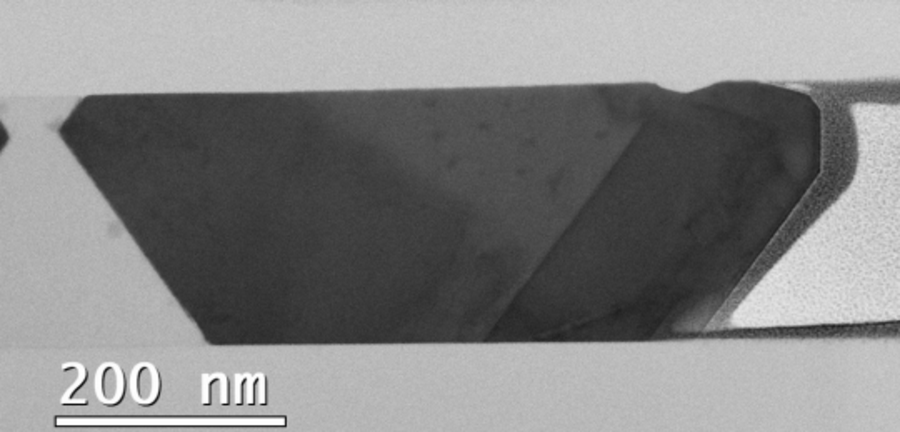
\includegraphics[width = \textwidth]{3_Growth/S2_right_overview.pdf}
    }
    \subcaptionbox{
        \acs{eds} map: red-\acs{in}, blue-\acs{ga} \cite{Brugnolotto2023}.
        \label{subfig:s2_III_ov_EDS}
    }{
        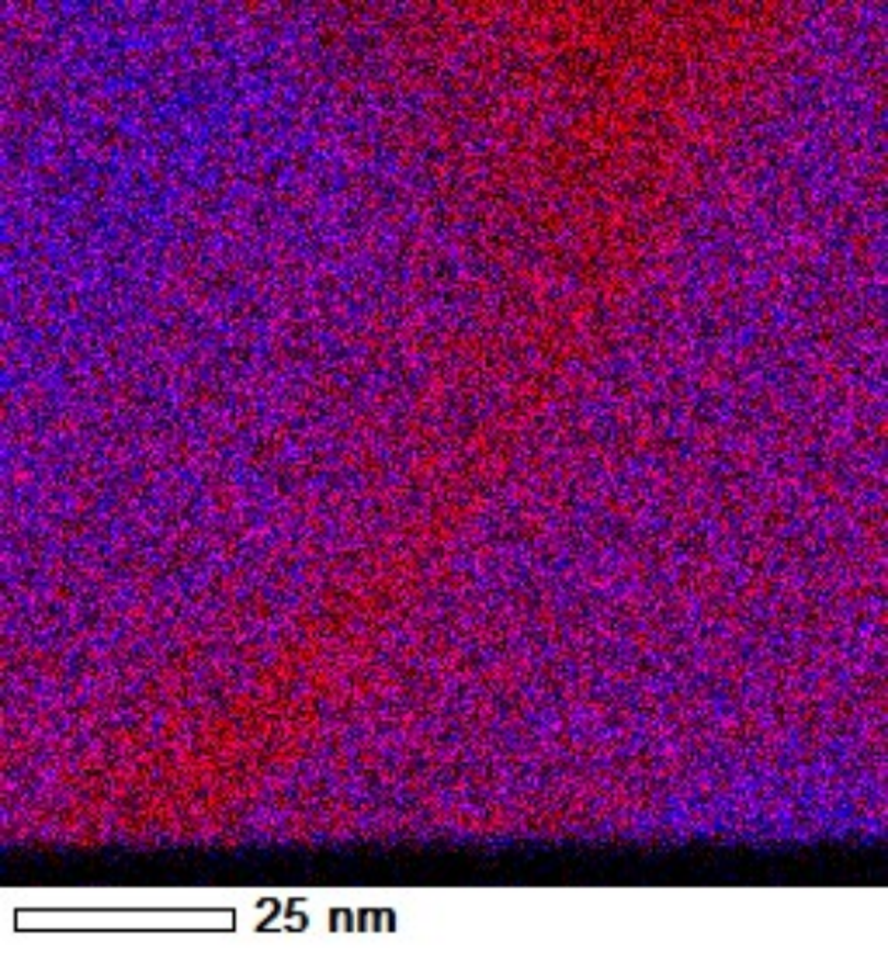
\includegraphics[width=0.45\textwidth]{3_Growth/s2_III_ov_EDS.pdf}
    }
    \subcaptionbox{
        \acs{eds} map: red-\acs{as}, blue-\acs{p} \cite{Brugnolotto2023}.
        \label{subfig:s2_V_ov_EDS}
    }{
        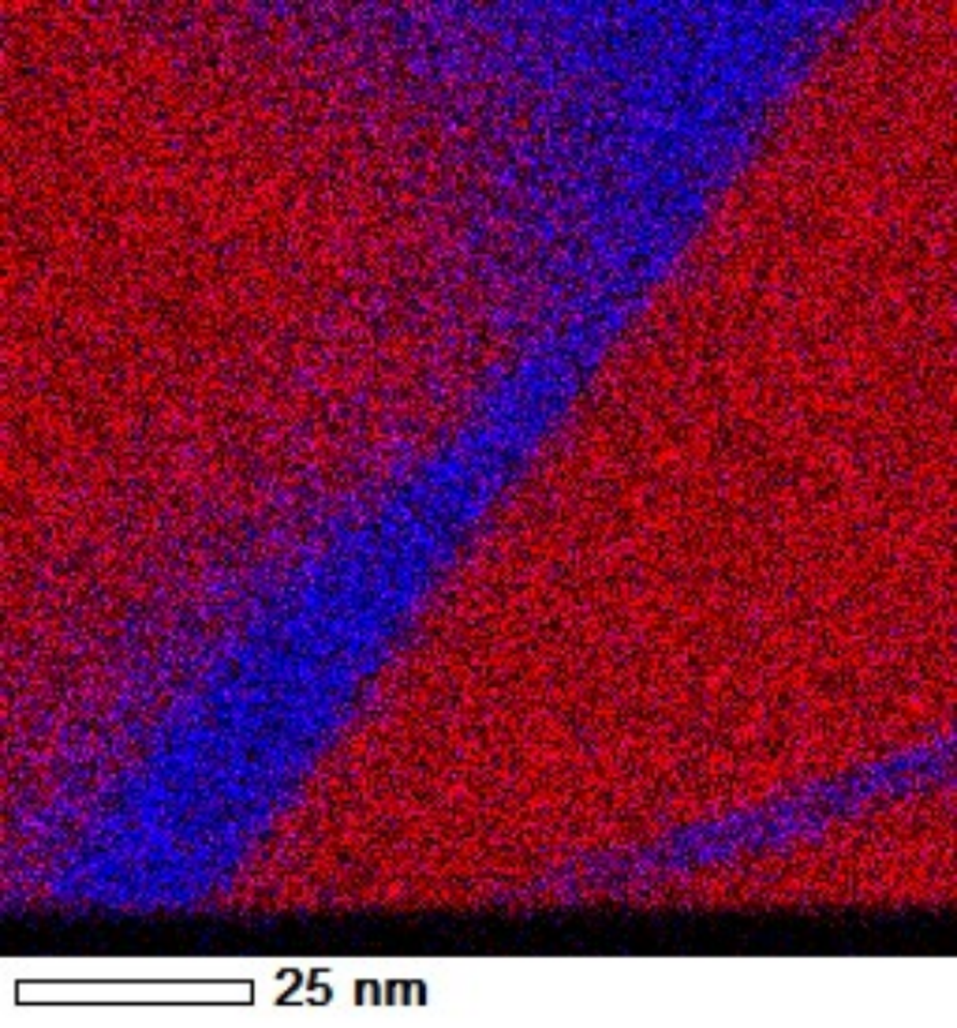
\includegraphics[width=0.45\textwidth]{3_Growth/s2_V_ov_EDS.pdf}
    }
    \caption[\acs{bf}-\acs{stem_m} overview image of a nanowire cross section with \acs{eds} maps.]{Microscopy images of the second sample. \subref{subfig:s2_r_ov} shows a \acs{bf}-\acs{stem_m} image of the lamella of sample 2, centred on the right wire. Various interfaces are visible, such as the \acs{si}/III-V interface and those between the two materials in the thick \acs{inp} and \acs{ingaas} layers. Some other areas of interest are also present. \subref{subfig:s2_III_ov_EDS} shows the III group element \acs{eds} map, and \subref{subfig:s2_V_ov_EDS} the V group element \acs{eds} map, of the lamella shown in \subref{subfig:s2_r_ov}.}
    \label{fig:sample2_stem}
\end{figure}

The \acs{stem_m} analysis of the sample started with the recording of the overview image in Figure~\ref{subfig:s2_r_ov}. It is a \acs{bf}-\acs{stem_m} image showing the right wire visible in Figure~\ref{subfig:FIB_cut_2}. The \acl{si} seed presents the previously discussed "V"-shaped interface composed of two \hkl{1 1 1} facets, which are once more identifiable by the image contrast on the left side of the image. A brighter region within the dark III-V material segment coincides with the presence of \acs{inp}. The evolution of the interfaces follows the trend that was highlighted in sample 1, with an initial \acs{ingaas} segment growing with a multi-faceted growth front exhibiting both \hkl{1 1 0} and \hkl{1 1 1} facets. The following \acs{inp} layer grows quickly in the \hkl{1 1 0} directions, and as such, the bottom \hkl{1 1 1} facet is larger. However, in the following segment, thinner material layers can no longer be identified through channelling-driven differences in contrast.
\par
\paragraph{Facet selection} The presence of two top \hkl{1 1 0} facets and the tendency of multiple facets of this family to form in this growth configuration is also reflected in the existing literature \cite{Borg2014, Schmid2015, Borg2015, Knoedler2017}. The initial nucleation sees the formation of a multi-faceted \acs{ingaas} particle resting on the \acl{si} seed surface. As it grows, the difference in growth rates of the different facets and the template walls limit which facets establish a stable growth front. Looking at the \hkl[1 1 0] growth axis in the cubic system, there are five energy-equivalent \hkl{1 1 0} facets available, of which the first is perpendicular to the template orientation and the other four's defining vector is offset by \qty{60}{\degree} from the first one's. On the other hand, there are only two available \hkl{1 1 1} facets at \qty{35.3}{\degree} close to the template direction. Furthermore, in the zincblende system, the \hkl{1 1 1} facets can be classified as \hkl{111}\(_A\) and \hkl{111}\(_B\) depending on whether only III or V atoms are exposed, respectively. The high V/III ratio loaded into the reactor during the \acs{inp} deposition step selects the \hkl{111}\(_B\) facet due to the marked prevalence of \acl{p} in the reactor atmosphere. The same \acl{p} saturation is likely to occur on the \hkl{1 1 0} facets; however, the difference in the morphology of the facet means that growth is enhanced on this facet, leading to its annihilation.

An example of how the different growth rates for each facet family affect the shape of the crystal is seen in the \acs{ingaas} layer immediately after this central \acs{inp} region. Here, growth appears to be relatively slow on \hkl{1 1 2} facets, and a void region is created at the top of the wire. Looking at Figure~\ref{subfig:FIB_cut_2}, this information confirms the interpretation of the darker region spotted at the top of the right wire on the upper \acs{sio2} template wall. This allows a better understanding of the shape of this void region: its limits are mainly perpendicular to the template axis, except in the area closest to the far template wall, where it appears that the limit closest to the seed curves back.
\par
\paragraph{Initial spectroscopic analysis} III and V group element EDS maps centred on the central \acs{inp} segment are shown in Figure~\ref{subfig:s2_III_ov_EDS} and \ref{subfig:s2_V_ov_EDS} respectively. Once again, the thick \acs{inp} layer already identified through channelling contrast is immediately noticeable at the centre of the images. However, the V map in Figure~\ref{subfig:s2_V_ov_EDS} also shows an important clue to the location of one of the heterointerfaces in the thin layer segment at the end of the wire. A small blue line is visible on the bottom right of this image, revealing the presence of \acl{p} in this wire area. This phosphide layer originated from the \qty{75}{\second} long pulse in the looped segment of the recipe shown in Figure~\ref{subfig:recipe2} and is well defined, without shading at the edges, which means that the growth front facet was perpendicular to the viewing direction. Despite this, no corresponding \acs{in}-rich layer is found in Figure~\ref{subfig:s2_III_ov_EDS}. This finding points to a difference in the relationship between precursor flow and elemental incorporation during material growth for the III and the V group elements when the growth occurs in templates.
\par


\begin{figure}
    \centering
    \subcaptionbox{
        High-Res \acs{bf}-\acs{stem_m} image of the \acs{inp} layer \cite{Brugnolotto2023}.
        \label{subfig:s2_thick_heterostructure}
    }{
        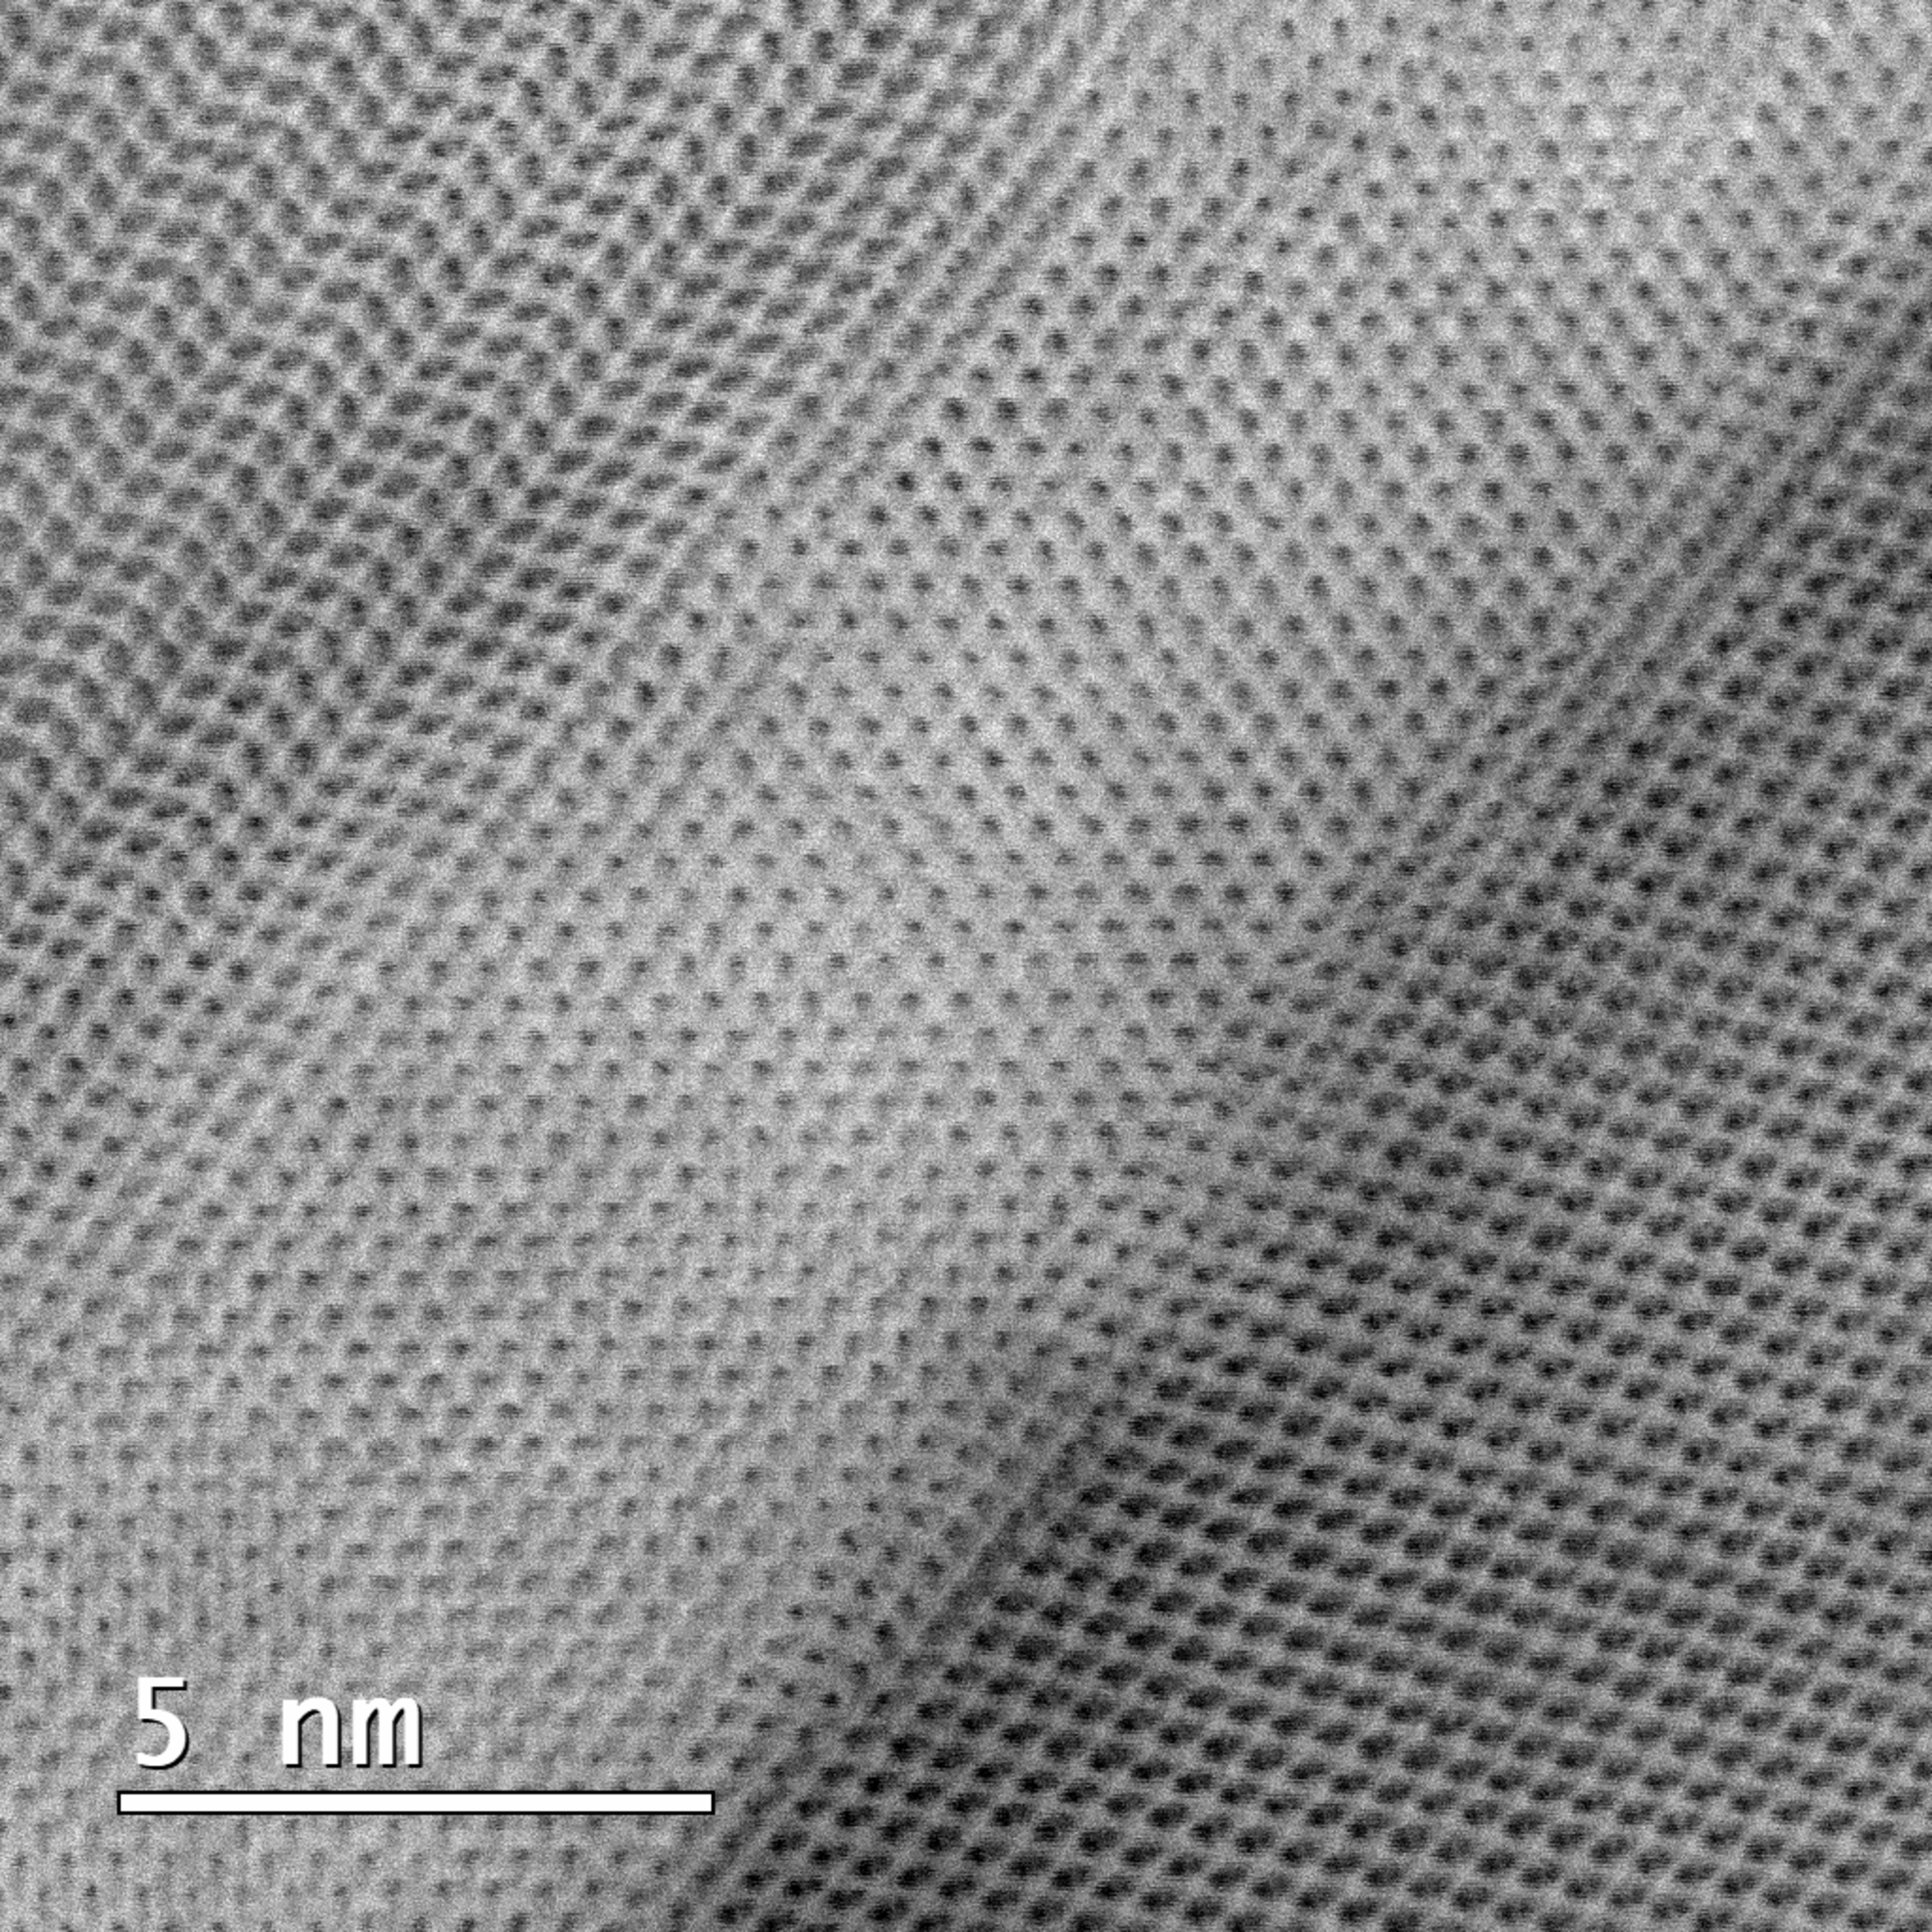
\includegraphics[width=0.45\textwidth]{3_Growth/s2_thick_Heterostructure.pdf}
    }
    \subcaptionbox{
        High-Res \acs{bf}-\acs{stem_m} image of the III-\acs{p} layer.
        \label{subfig:s2_V_thin_heterostructure}
    }{
        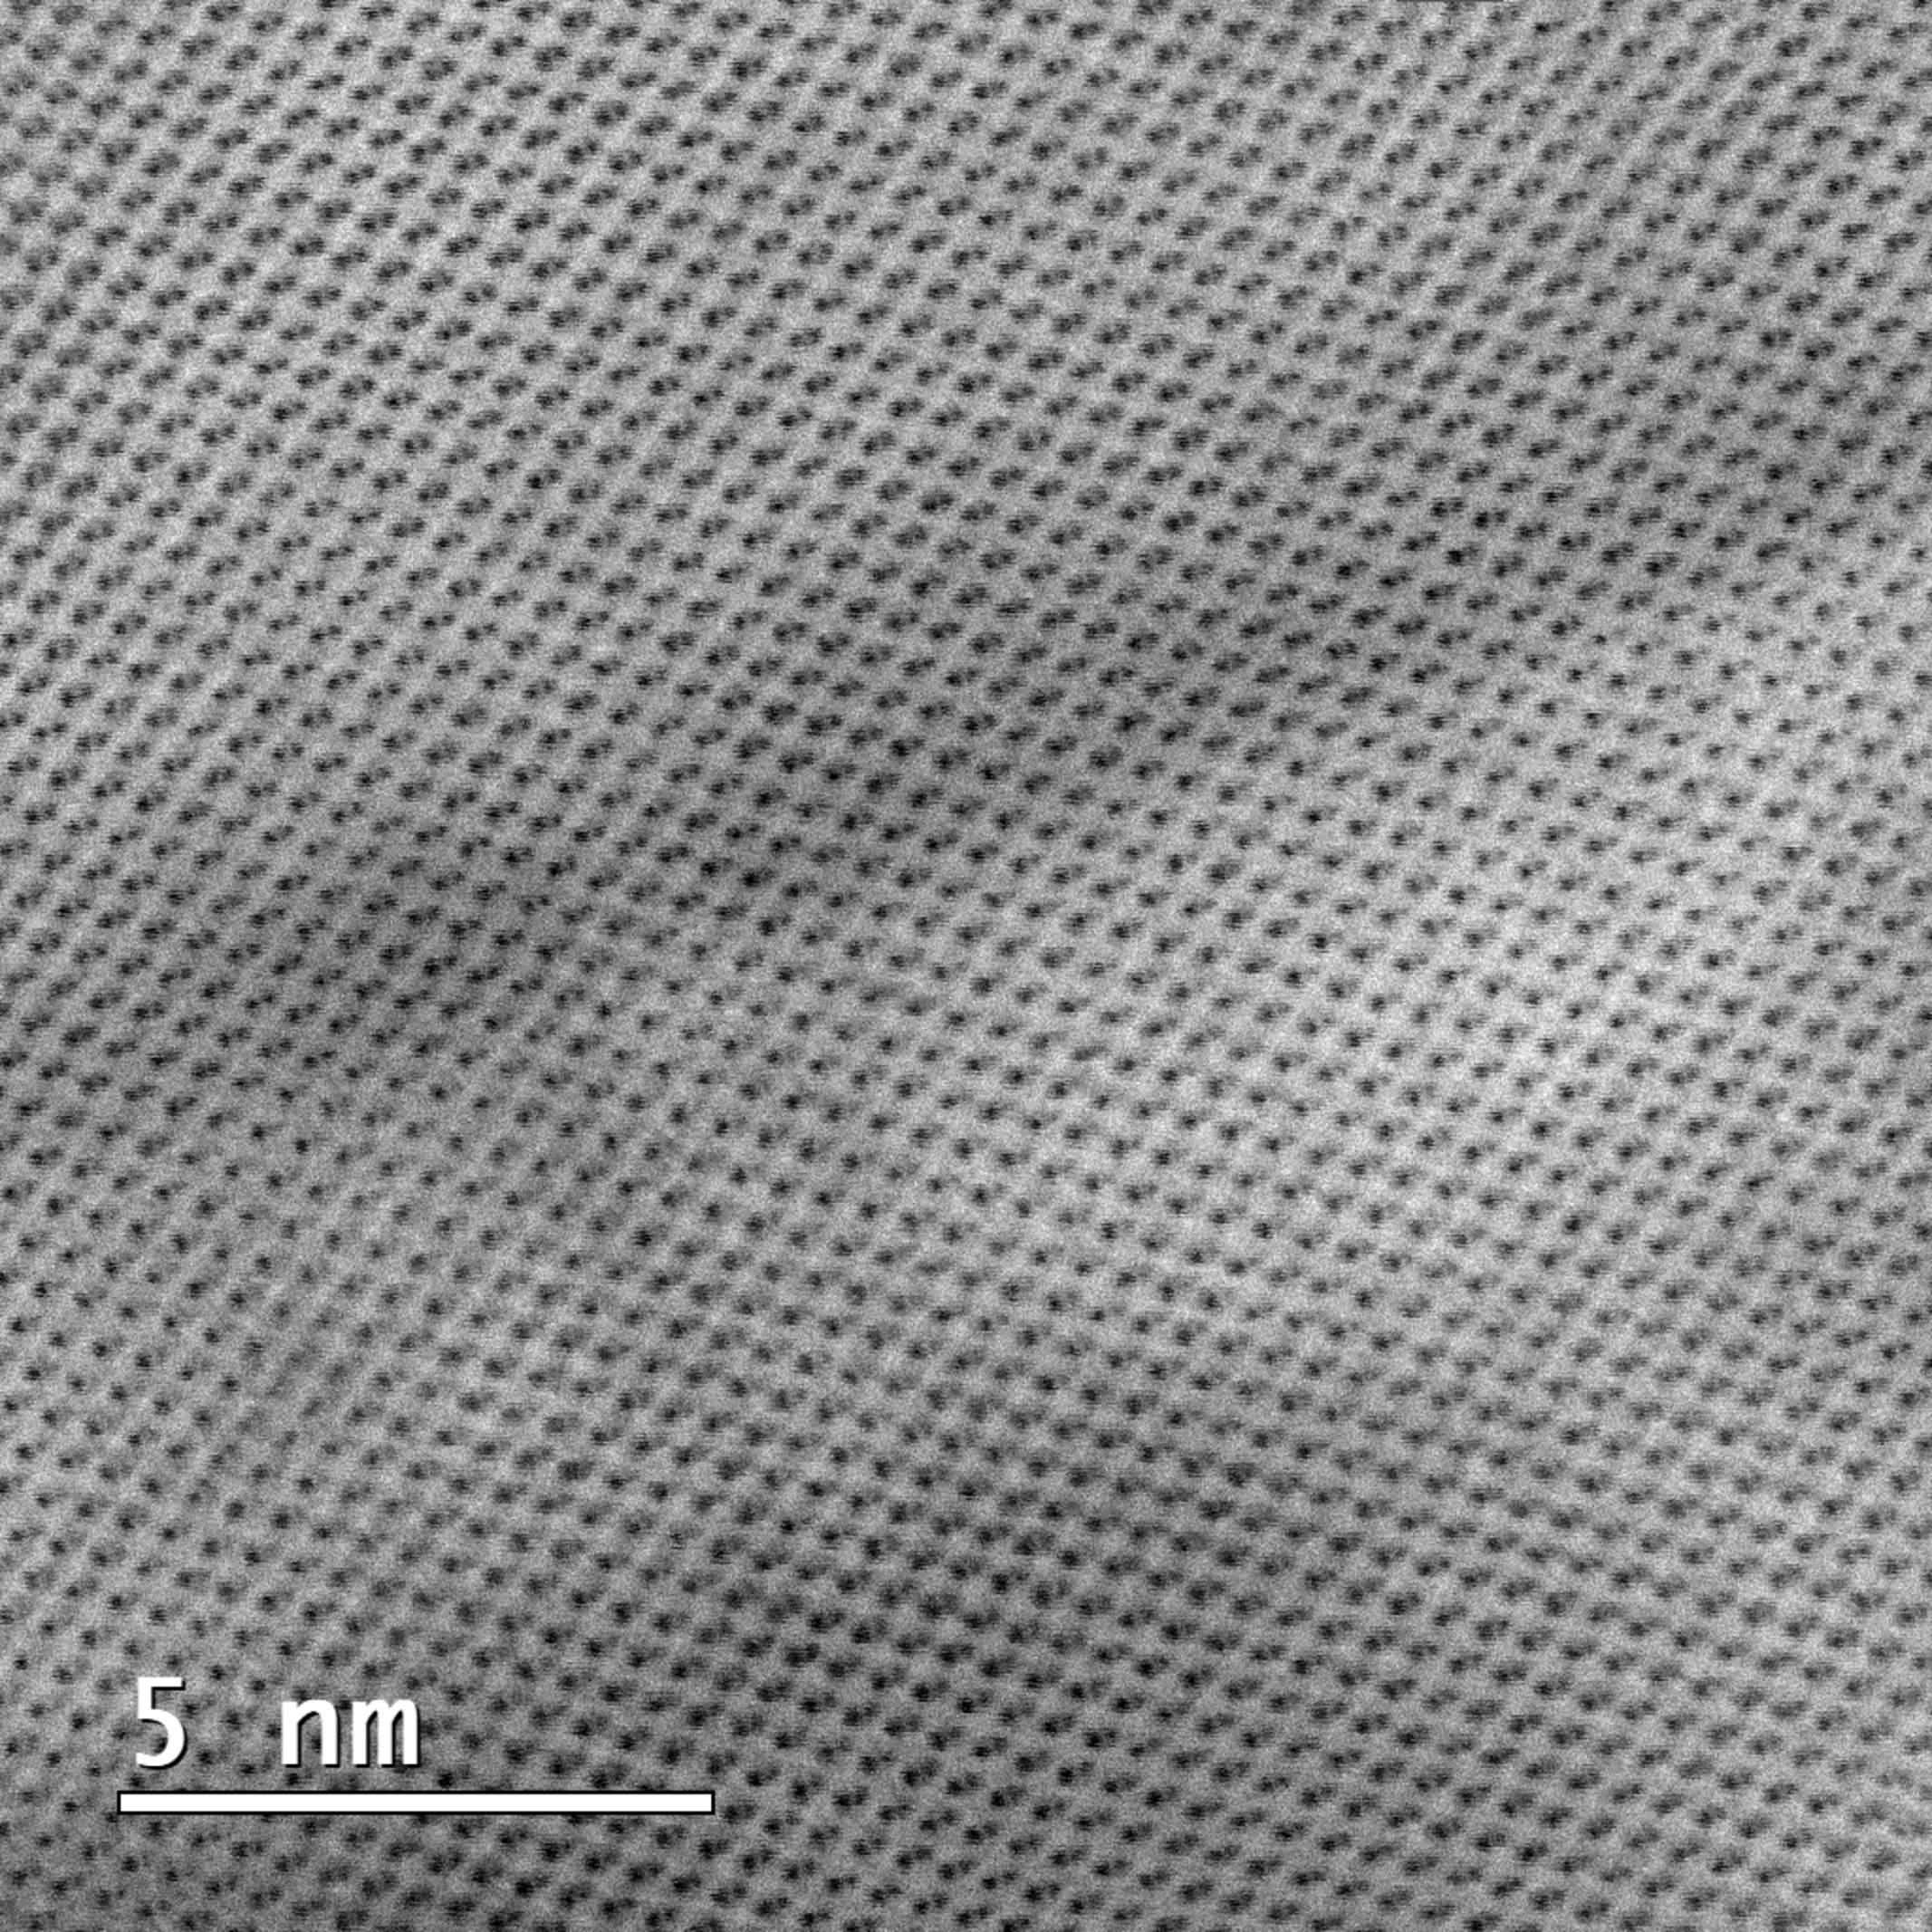
\includegraphics[width=0.45\textwidth]{3_Growth/s2_thin_Heterostructure.pdf}
    }
    \subcaptionbox{
        \acs{eds} map of the \acs{p} concentration.
        \label{subfig:s2_int2_P}
    }{
        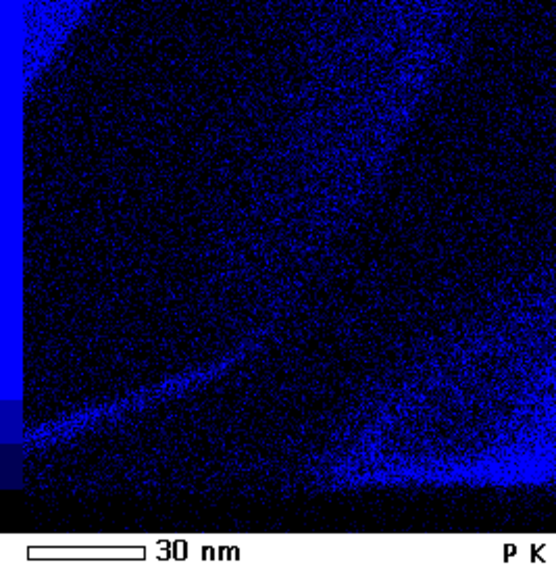
\includegraphics[width=0.45\textwidth]{3_Growth/s2_int2_P.pdf}
    }
    \subcaptionbox{
        \acs{eds} map of the \acs{in} concentration.
        \label{subfig:s2_int2_In}
    }{
        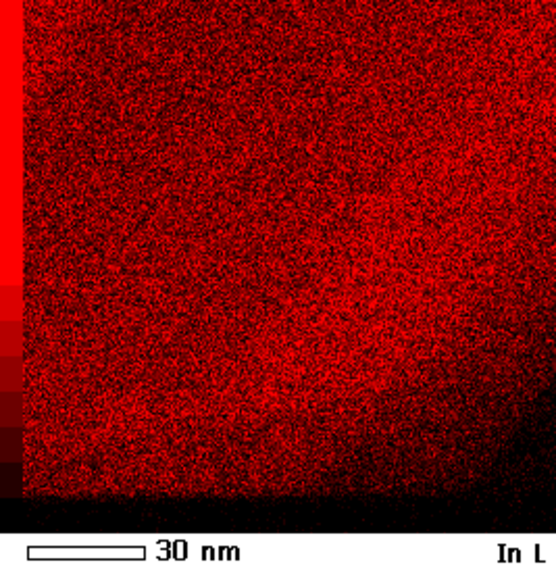
\includegraphics[width=0.45\textwidth]{3_Growth/s2_int2_In.pdf}
    }
    \caption[High-resolution \acs{bf}-\acs{stem_m} images and \acs{eds} maps of \acs{in} and \acs{p} in the area grown to contain thin material layers in sample 2.]{Analysis of the thin-layer region. \subref{subfig:s2_thick_heterostructure} \acs{bf}-\acs{stem_m} image of the lower part of the thick \acs{inp} layer, where it is at its thinnest. \subref{subfig:s2_V_thin_heterostructure} \acs{bf}-\acs{stem_m} image of the thin phosphide interface at the bottom left of \ref{subfig:s2_r_ov}. \subref{subfig:s2_int2_P} \acs{eds} composition map of \acl{p} presence in the sample. \subref{subfig:s2_int2_In} \acs{eds} composition map of \acl{in} presence in the sample.}
    \label{fig:s2_details}
\end{figure}

\paragraph{High-resolution imaging} Two high-resolution \acs{bf}-\acs{stem_m} images of the phosphide segments identified in the spectroscopic analysis of the sample are presented in Figure~\ref{subfig:s2_thick_heterostructure} and \ref{subfig:s2_V_thin_heterostructure}. Figure~\ref{subfig:s2_thick_heterostructure} shows the layer resulting from the long \acs{inp} deposition step sandwiched between two \acs{ingaas} segments. The two materials are easily distinguishable, as the III-\acs{as} couples have similar sizes for both atoms. In contrast, the \acl{p} atoms are much smaller and are almost invisible next to the \acl{in} atoms in the \acs{inp} region. \acl{rtp}s are visible on the top left of the image, in the \acs{ingaas} layer. However, they are not visible after the \acs{inp} layer in the next \acs{ingaas} layer. This, coupled with the presence of \hkl{1 1 2} facet in the growth front, could indicate that something is affecting the growth of the wire after this point: precisely what cannot be analysed easily after the growth itself is complete. Therefore, it becomes prudent to avoid drawing conclusions about the shape of the growth front morphology after this area. However, an analysis of how the III and V composition profiles interact is still possible, as this is related to the diffusion of the precursor in the template. Further, the thickness of the phosphide layer in Figure~\ref{subfig:s2_V_thin_heterostructure} is \qty{6}{nm}, indicating the potential for thin heterostructures with well-defined composition gradients. 

\paragraph{Further spectroscopic analysis} The ending region of the wire was further analysed with \acs{eds}, resulting in the two images in Figure~\ref{subfig:s2_int2_P} and \ref{subfig:s2_int2_In}. They show the concentration profiles calculated from the signal intensity at the \acl{p} K line and \acl{in} L line, respectively. As discussed during the analysis of the previous sample, the \acl{p} K\(_\alpha\) line is very close in energy to the \acl{pt} M line. Therefore, the high \acl{p} signal visible on the bottom right of the image is interpretable as \acl{pt} presence. 

This comparison aims to evaluate the growth of the \acs{inp} segment based on how the \acl{in} and \acl{p} concentrations line up in the sample. As is particularly evident from observing the top right corners of each \acs{eds} map, the area with high \acl{in} concentration is to the left of the one with high \acl{p} concentration. This indicates a delay in III group element integration compared to the corresponding V group element integration step. This is likely due to a difference in diffusion between the two materials and will need to be solved if precise integration of thin III-V material layers is to be attempted.

The complex layer morphology and, most importantly, the high composition intermixing between material layers make it impossible to calculate growth rates for this terminal area of the wire.

\subsection{Correlation between growth dynamics and results}
Figure~\ref{fig:issues} summarises the four main findings from the first two samples, which were grown using relatively simple \acs{mocvd} recipes. The stabilisation of the \hkl{1 1 1} facet in high V/III ratio \acs{inp} deposition makes this combination of material and facet the preferred one for the growth of thin heterostructures. The potential for thin hetero layers and \acl{qw}s was highlighted by the \qty{6}{\nano\metre} wide phosphide structures shown in the second sample. The thickness of the \acs{inp} layer in Figure~\ref{subfig:s2_thick_heterostructure} can be misleading, as without the context given by the larger overview image in Figure~\ref{subfig:s2_r_ov}, the information is lost that most of the material deposition occurs on the \hkl{1 1 0} facets. 
\par
Still, both Figure~\ref{subfig:s2_thick_heterostructure} and Figure~\ref{subfig:s2_V_thin_heterostructure} show that for the V component of the semiconductor, it is possible to obtain <\qty{10}{\nano\metre} thick compositional structure. However, for the III group elements, short deposition pulses lead to heavy alloying and delay in integration. This indicates the presence of different diffusion mechanisms that affect the supply of reactant to the reaction interface (the growth front). 

When the possible diffusive pathways available to the precursors are examined, it becomes clear that gas-phase diffusion is the first route available directly from the showerhead, through which precursors are introduced into the reactor. However, when the precursors land on the wafer, the surface is non-reactive, unlike in planar growth, and the adsorbed precursors either desorb and continue diffusion through the gas phase or diffuse on the surface to reach the reaction interface. If the V precursors mainly desorb from the surfaces and the majority of them get the reaction interface through gas-phase diffusion, and if the III precursors tend to diffuse as adsorbates on the surface, then this could be the diffusive mechanism difference that can explain the different sharpnesses in heterointerfaces. Additionally, if it is assumed that adsorbate diffusion is a slower mechanism than vapour phase diffusion, then this could also explain the integration delay of III group elements compared to their expected layer. 

These two diffusion routes are illustrated in Figure~\ref{subfig:diffusion_mechanisms}. Given the small volume of the cavities, Knudsen vapour phase diffusion occurs inside the template. This diffusion regimen appears when the mean free path of the diffusing element is comparable to the size of the area within which it is diffusing. Simultaneously, the III group elements diffuse inside the template with the additional mechanism of adsorbate diffusion. This means that the III atoms can jump from equilibrium to equilibrium site on the surface of the template oxide until they reach the reaction interface. The effects of the different availability of these diffusion pathways to the various species are highlighted for short deposition pulses as the deposition time approaches the diffusion timescales \cite{Brugnolotto2023}.

\begin{sidewaysfigure}
    \centering
    \subcaptionbox{
        The main findings from the first two samples are represented schematically. From left to right, the stabilisation of the \hkl{1 1 1} growth front during \acs{inp} growth, the thin phosphide heterolayers, III group element composition intermixing, and the diffusion-driven integration delay are shown.
        \label{fig:issues}
    }{
        
\includegraphics[width=0.45\textwidth]{3_Growth/issues.pdf}
    }
    \subcaptionbox{
    Diffusion mechanisms inside the \acs{sio2} interface. Bulk materials are labelled, with the two \acs{sio2} template layers above and below the III-V wire. The precursors are represented by black (III group element precursors) and grey (V group element precursors) circles. \cite{Brugnolotto2023}.
    \label{subfig:diffusion_mechanisms}
    }{
        \tikzsetnextfilename{diffusion_mechanisms}
        \begin{tikzpicture}
            \filldraw[fill=red] (0cm, 0cm) -- node[midway, anchor = west] {III-V} (0cm, 22mm) -- (2cm, 22mm) -- ++ (-54.7:2.8cm) --  cycle;
            \filldraw[fill=SiO2_blue] (0cm, -10mm) -- (11cm, -10mm) -- (11cm, 0cm) -- (0cm, 0mm) --  node[midway, anchor=west] {\acs{sio2}} cycle;
            \filldraw[fill=SiO2_blue] (0cm, 22mm) -- (11cm, 22mm) -- (11cm, 32mm) -- (0cm, 32mm) --  node[midway, anchor=west] {\acs{sio2}} cycle; 
            \filldraw[fill=black] (7, 1.5) circle (1mm) node [anchor = west] {Knudsen diffusion};
            \draw[-stealth] (6.85, 1.5) -- (6.65, 1.5);
            \draw[dotted, thick] (6.5, 1.5) circle (1mm);
            \filldraw[fill=gray] (6, 1.5) circle (1mm);
            \draw[-stealth] (5.85, 1.5) -- (5.65, 1.5);
            \draw[gray, dotted, thick] (5.5, 1.5) circle (1mm);
            \filldraw[fill=black] (7, 0.1) circle (1mm) node [anchor = south west] {Adsorbate diffusion};
            \draw[-stealth] (6.9, 0.17) arc[start angle = 45, end angle = 125, radius = 0.25];
            %\draw[-stealth] (6.85, 0.1) -- (6.65, 0.1);
            \draw[dotted, thick] (6.5, 0.1) circle (1mm);
            %\draw (3.2cm, 22mm) arc [start angle = 180, end angle = 324.7, radius = 3mm] node[midway, anchor = north east]{\qty{144.7}{\degree}};
            %\draw[-stealth] (8cm, 7mm) node[anchor=north] {\hkl<1 -1 0>} -- ++ (90:0.8cm) node[anchor=south] {\hkl<0 0 1>};
            %\draw[-stealth] (8cm, 7mm) -- ++ (0:0.8cm) node[anchor=west] {\hkl<1 1 0>};
            %\node[mark size=2pt] at (8, 7mm) {\pgfuseplotmark{diamond*}};
        \end{tikzpicture}
    }
    \subcaptionbox{
        Growth recipe for sample 3 \cite{Brugnolotto2023}. Each line represents an active flow of the corresponding precursor into the reactor. The colour of the horizontal lines represents the target material.
        \label{subfig:recipe3}
    }{
        \tikzsetnextfilename{recipe3}
        \begin{tikzpicture}
            \begin{scope}
            % lines
                \node [label={[label distance=0]180:\acs{in}}] at (0, 0) {};
                \draw [red, ultra thick, dashed] (0, 0) -- (4.8, 0); %/10
                \draw [cb1_dark_blue, ultra thick, dashed] (4.8, 0) -- (6.6, 0); %10
                \draw [cb1_orange, ultra thick] (8.6, 0) -- (11.6, 0);
                \draw [cb1_dark_blue, ultra thick, dashed] (13.6, 0) -- (15.4, 0); %10
                %\draw [cb1_orange, ultra thick] (7.35, 0) -- (8.1, 0);
        
                \node [label={[label distance=0]180:\acs{ga}}] at (0, -0.5) {};
                \draw [red, ultra thick, dashed] (0, -0.5) -- (4.8, -0.5cm); %/10
                \draw [cb1_orange, ultra thick] (8.6, -0.5) -- (11.6, -0.5);
        
                \node [label={[label distance=0]180:\acs{as}}] at (0, -1) {};
                \draw [red, ultra thick, dashed] (0, -1) -- (4.8, -1); %/10
                \draw [cb1_orange, ultra thick] (8.6, -1) -- (11.6, -1);
                \draw [gray, ultra thick] (11.6, -1) -- (13.1, -1);
        
                \node [label={[label distance=0]180:\acs{p}}] at (0, -1.5) {};
                \draw [cb1_dark_blue, ultra thick, dashed] (4.8, -1.5) -- (6.6, -1.5); %/10
                \draw [gray, ultra thick] (6.6, -1.5) -- (8.6, -1.5);
                \draw [gray, ultra thick] (13.1, -1.5) -- (13.6, -1.5);
                \draw [cb1_dark_blue, ultra thick, dashed] (13.6, -1.5) -- (15.4, -1.5); %/10
                \draw [gray, ultra thick] (15.4, -1.5) -- (17.4, -1.5);
        
            % labels and markers for the timescale
                \node [label={[label distance=0]180:Time (\second)}] at (0, -2) {};
                \draw [dashed] (0, -2) -- (6.6, -2);
                \draw [] (6.6, -2) -- (13.6, -2);
                \draw [dashed] (13.6, -2) -- (15.4, -2);
                \draw [-stealth] (15.4, -2) -- (17.7, -2);
                \draw [] (0, 0.2) -- (0, -2.2) node[anchor = north] {\num{0}};
                \draw [] (4.8, 0.2) -- (4.8, -2.2) node[anchor = north] {\num{480}};
                \draw [] (6.6, 0.2) -- (6.6, -2.2) node[anchor = north] {\num{660}};
                \draw [] (8.6, 0.4) -- (8.6, -2.2) node[anchor = north] {\num{680}};
                \draw [] (11.6, 0.2) -- (11.6, -2.2) node[anchor = north] {\num{710}};
                \draw [] (13.1, 0.2) -- (13.1, -2.2) node[anchor = north] {\num{725}};
                \draw [] (13.6, 0.2) -- (13.6, -2.8) node[anchor = north] {\num{730}};
                \draw [] (15.4, 0.2) -- (15.4, -2.2) node[anchor = north] {\num{910}};
                \draw [] (17.4, 0.4) -- (17.4, -2.2) node[anchor = north] {\num{930}};
                \draw [stealth - stealth] (8.6, 0.3) -- (17.4, 0.3) node[midway, anchor=south] {Looped Recipe Segment  (x\num{2})};
            \end{scope}
                \begin{scope} [shift={(18.6cm, -0.5)}]
                \draw [gray, ultra thick] (0, 0.5) -- (0.5, 0.5) node[anchor = west, text=black] {Hold Step};
                \draw [cb1_orange, ultra thick] (0, 0) -- (0.5, 0) node[anchor = west, text=black] {\acs{ingaas}};
                \draw [cb1_dark_blue, ultra thick] (0, -0.5) -- (0.5, -0.5) node[anchor = west, text = black] {\acs{inp}};
                \draw [dashed, ultra thick] (0, -1) -- (0.5, -1) node[anchor = west, text = black] {\num{0.1} time scale};
                \draw (-0.3, 1) -- (3.3, 1) -- (3.3, -1.65) -- node[midway, fill = white] {Legend} (-0.3, -1.65) -- cycle;
            \end{scope}
        \end{tikzpicture}
    }
    \caption[Motivation and changes to the growth recipe with the introduction of hold steps for the growth of sample 3.]{\subref{fig:issues} Summary of insight from the first two growth runs. \subref{subfig:diffusion_mechanisms} Schematic representation of the diffusion avenues available inside the \acs{tase} template. \subref{subfig:recipe3} Modified \acs{mocvd} recipe based on the analysis of growth results.}
    \label{fig:s3_hold_steps}
\end{sidewaysfigure}

\section{Implementation of a revised switching sequence}
\label{sec:s3}

To address the intermixing and integration delay issues identified in Figure~\ref{fig:issues}, several modifications were made to the \acs{mocvd} growth recipe, resulting in the revised step sequence shown in Figure~\ref{subfig:recipe3}. In this graphic, the segments drawn with dashed lines are represented with a \num{0.1} time scale to maintain a reasonable size for the picture. The main additions to the recipe are the "hold steps": moments at the end of each layer deposition segment when the flow of III precursors was halted, leaving only a V group element atmosphere in the background. The \qty{5}{s}-long \acl{p} hold step was introduced after the \acl{as} hold step and the \acs{ingaas} deposition step in the looped recipe segment to promote a change in the atmosphere inside the template for the following \acs{inp} deposition step. The rationale for its introduction here but not in the previous arsenide-to-phosphide step is that the smaller size and weight of the \acl{p} atom would give it a higher mobility and a lower chance to diffuse as an adsorbate compared to the bulkier, heavier \acl{as} atom. 

A second modification affected the length of the material deposition segments, which was adjusted to consider the lower growth rate of \acs{inp} compared with \acs{ingaas}. As the looped segment was repeated twice for the next growth run, this recipe will theoretically result in the correct barrier/well material layers alternating to create two \acs{ingaas} \acl{qw}s in series in a \acs{inp} matrix. The V/III ratios and the \qty{580}{\degreeCelsius} growth temperature are kept constant to continue to benefit from the stabilisation of the single \hkl{1 1 1} facet growth front that occurs during \acs{inp} deposition.

The \acs{sem_m} image of the sample during \acs{fib} processing for \acs{stem_m} analysis was already shown in Figure~\ref{subfig:FIB_cut}. A hint of the finer structure is already visible by tracking the position of the \acl{in} droplets on the exposed \acs{inp} lateral surfaces.

\subsection{\texorpdfstring{\acs{stem_m} analysis}{STEM analysis}}

\begin{figure}
    \centering
    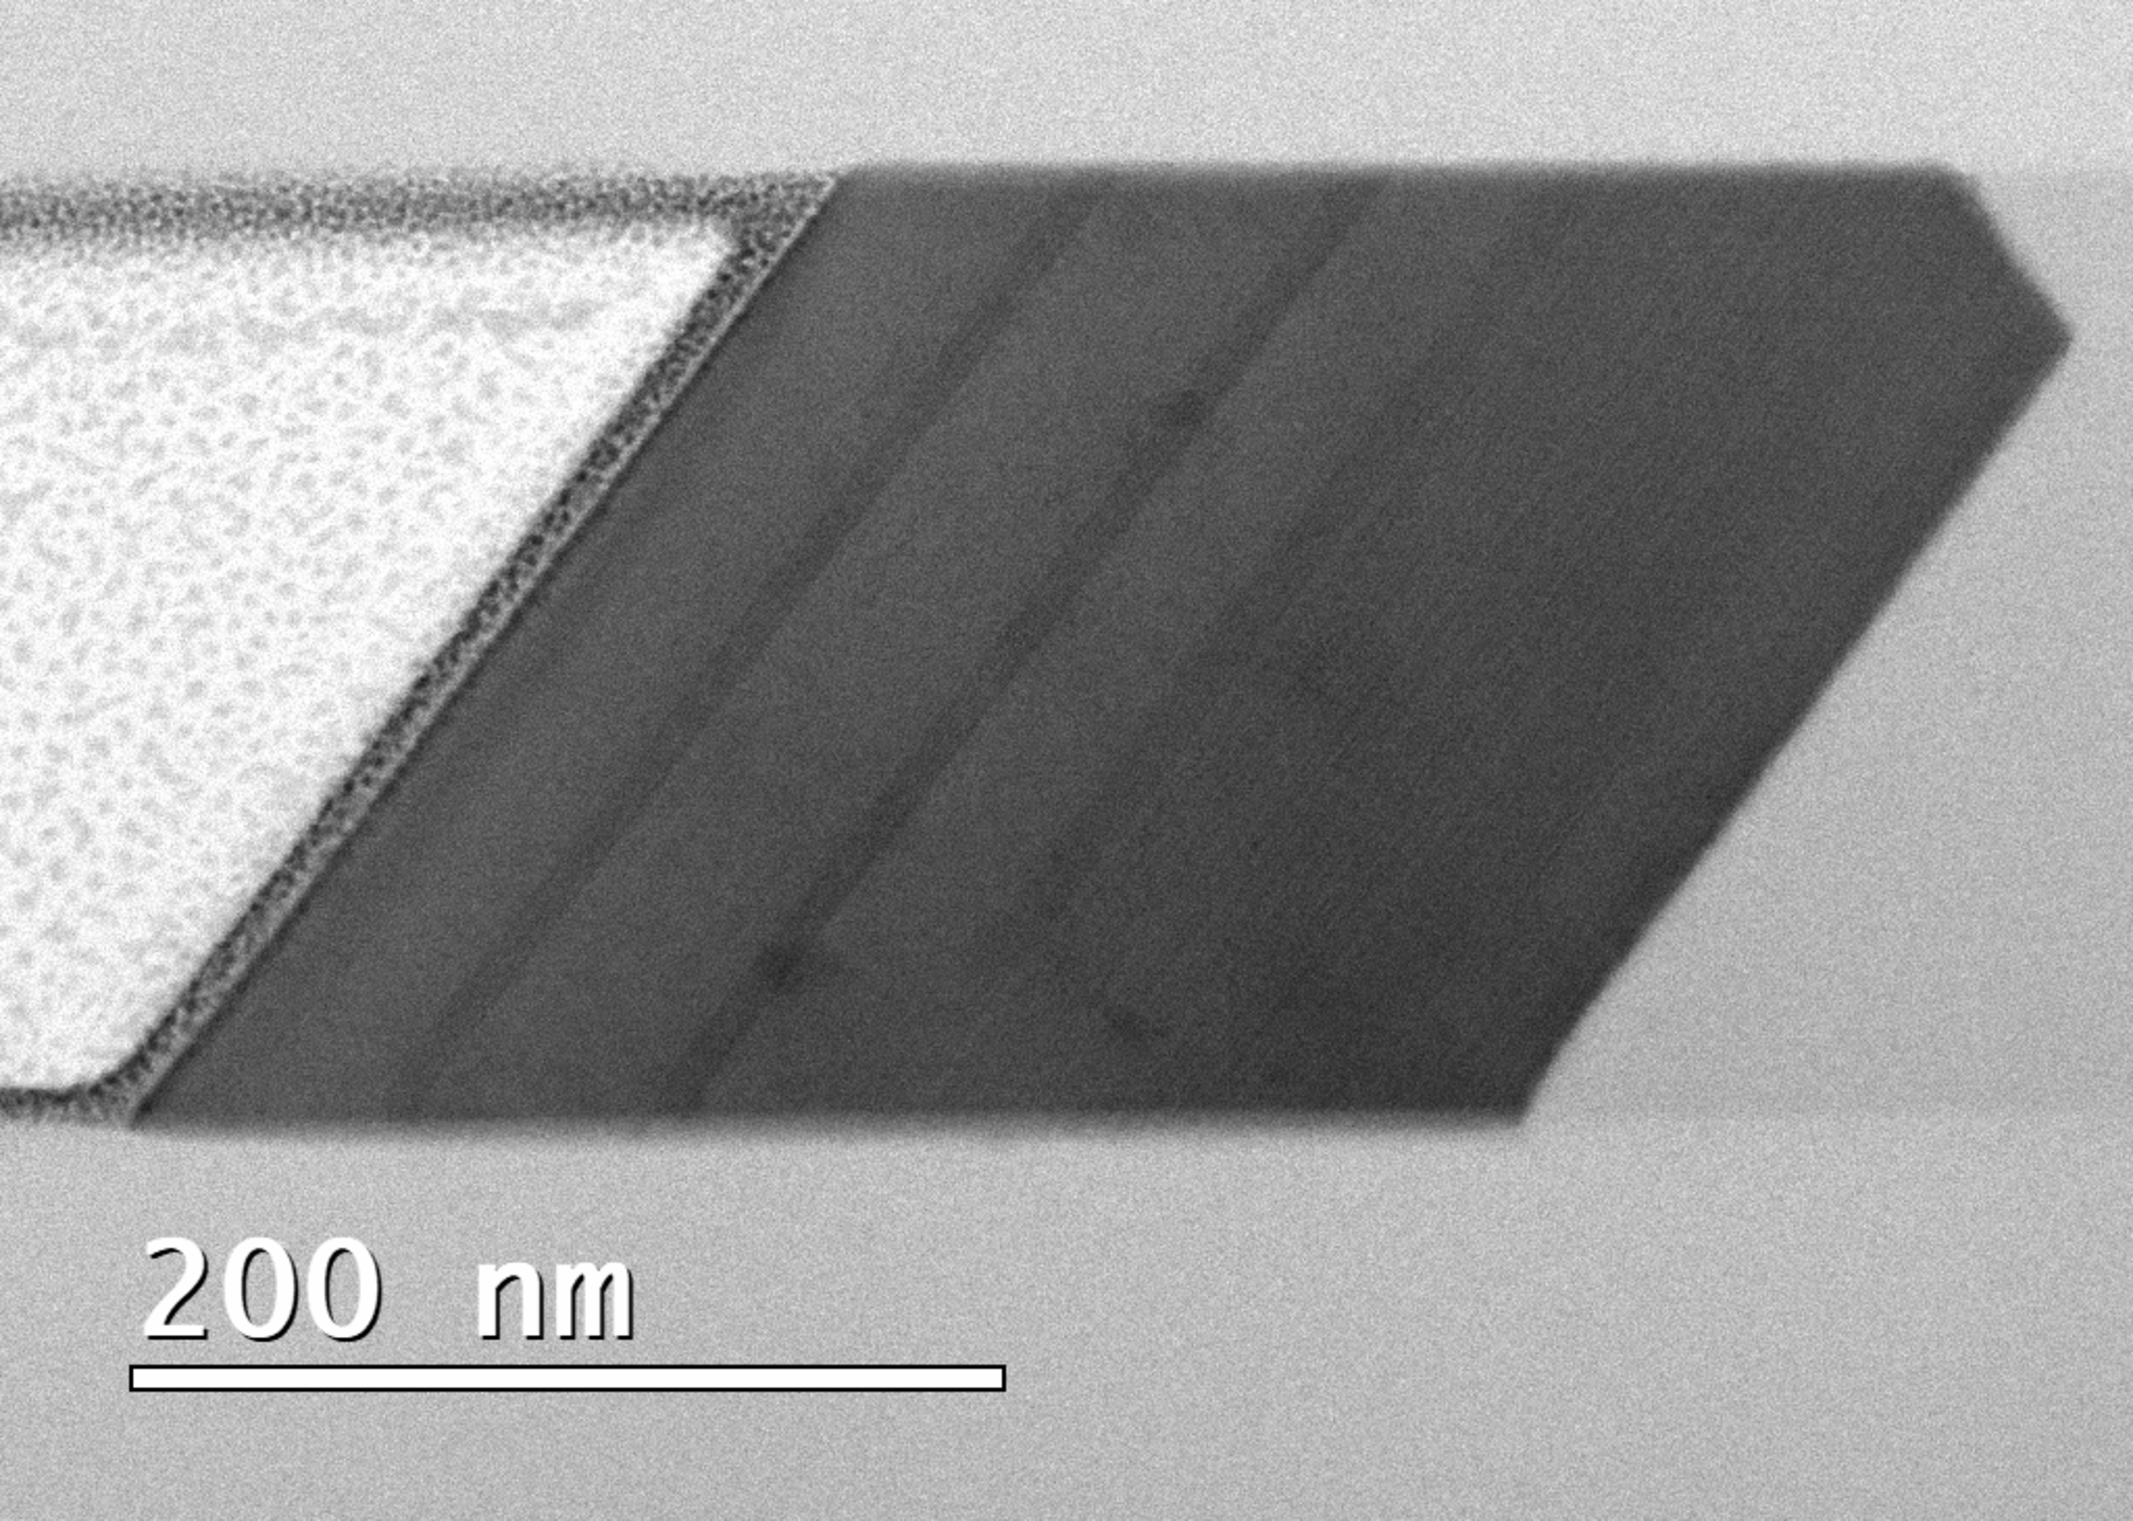
\includegraphics[width=\textwidth]{3_Growth/s3_ov.pdf}
    \caption[\acs{bf}-\acs{stem_m} image of a semiconductor lamella cut from a nanowire in sample 3.]{\acs{bf}-\acs{stem_m} image of a semiconductor lamella cut from a nanowire in sample 3 \cite{Brugnolotto2023}. The different material layers are already visible through channelling contrast.}
    \label{fig:s3_ov}
\end{figure}

The \acs{bf}-\acs{stem_m} image in Figure~\ref{fig:s3_ov} gives a better view of the material layers. The wire grew right-to-left from the \acl{si} seed on the right of the image, which, once again, has the "V" shaped morphology observed in the two previous samples. Then, from right to left, the first dark area consists of an \acs{ingaas} layer, followed by a lighter \acs{inp} layer and then by an alternating \acs{ingaas} and \acs{inp} well-barrier \acl{qw} structure. Compared to sample 2 (Figure~\ref{subfig:s2_r_ov}), here the thin heterolayers are immediately visible before \acs{eds} mapping, directly from the \acs{bf}-\acs{stem_m} image.

\acl{pt} is visible in the opening to the left of the III-V wire. The top and bottom of the image are occupied by the upper and lower \acs{sio2} template and buried oxide layers, respectively. The first \acs{ingaas} layer presents a multi-faceted growth front once again, with an upper \hkl{1 1 1} facet and a \hkl{1 1 0} region at the bottom. The following \acs{inp} layer stabilises the \hkl{1 1 1} facet up to the last few nanometres at the bottom of the wire, where a small \hkl{1 1 0} facet survives, maintained through the next \acs{ingaas} layer which is, importantly, conformal to the previous \acs{inp} segment when it comes to the morphology of the growth front. It is only in the second \acs{inp} layer that a single \hkl{1 1 1} facet is stabilised. However, it is clear that, given a sufficiently thick \acs{inp} layer, growth front stabilisation will occur.

\begin{figure}
    \centering
    \tikzsetnextfilename{s3_QW_HR}
    \begin{tikzpicture}
        \node[inner sep=0pt] (image) at (0,0) {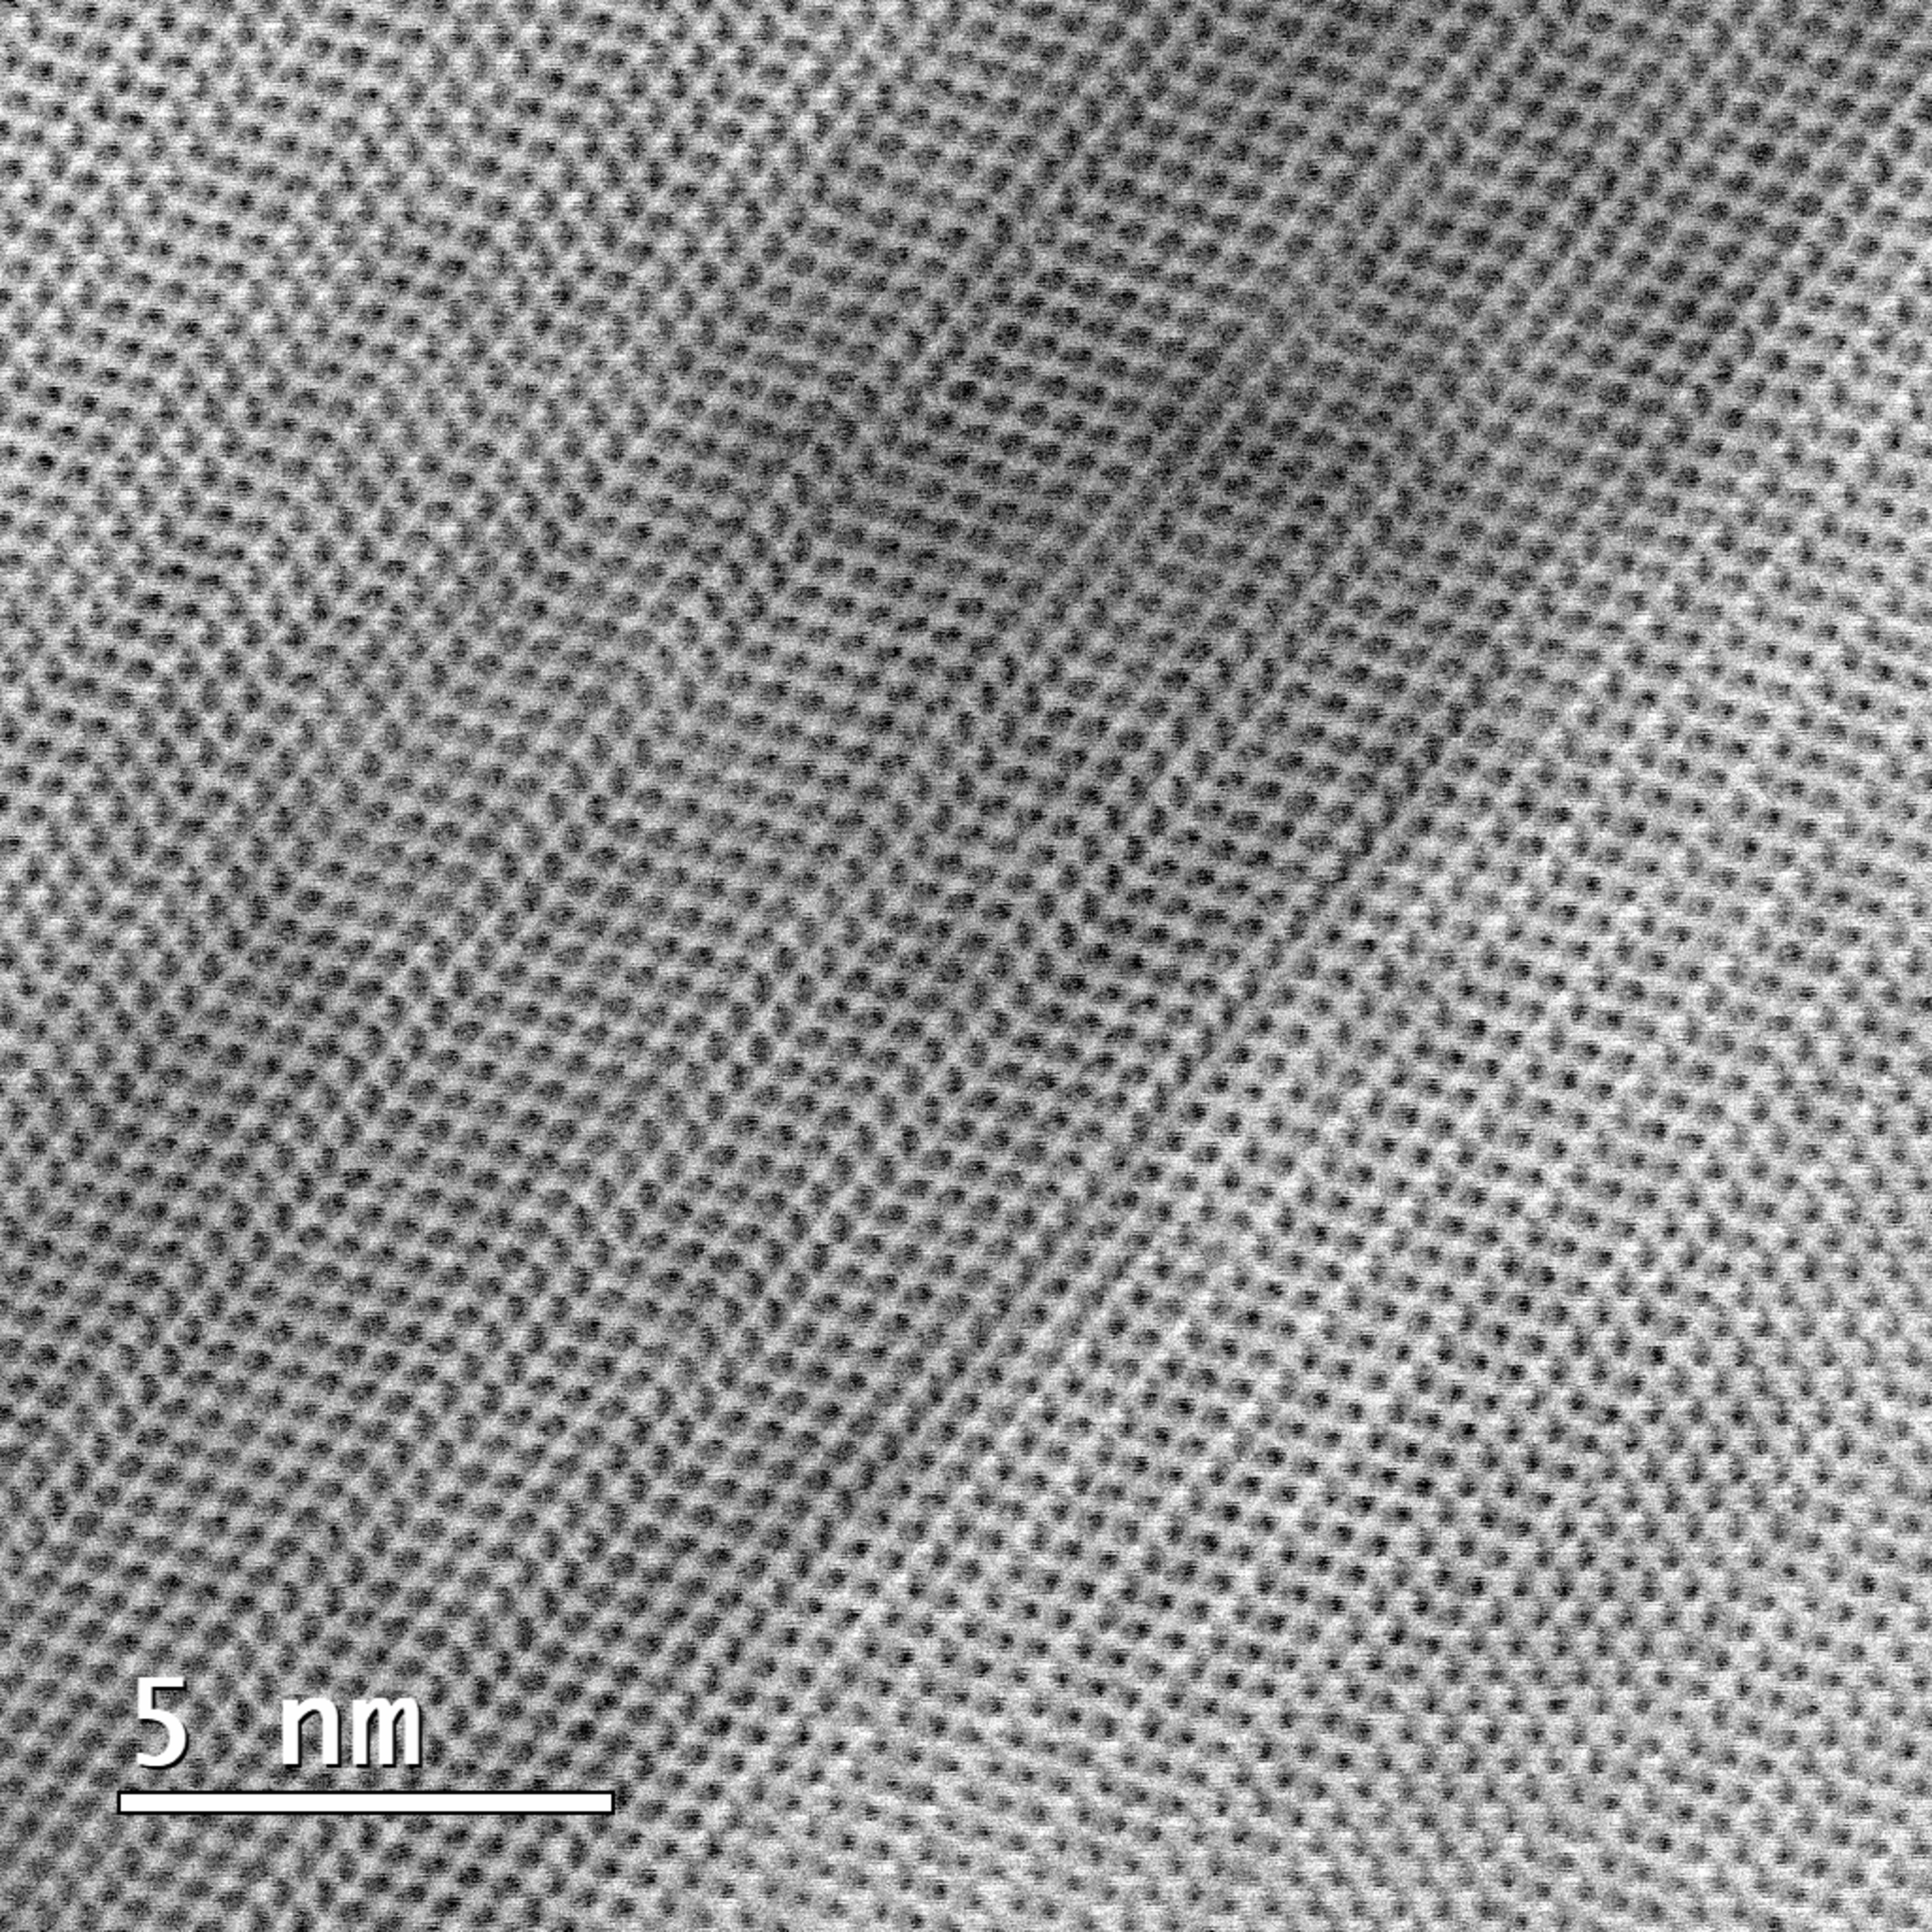
\includegraphics[width=0.5\textwidth]{3_Growth/s3_QW_HR.pdf}};
        \draw[red, thick, stealth-] (-2.5, 3) -- (3.5, -2.5) node[midway, rotate=-42, fill=white, anchor=south west]{EDS linescan};
    \end{tikzpicture}
    \caption[High-resolution \acs{bf}-\acs{stem_m} image of the second \acl{qw} region of sample 3.]{High-resolution \acs{bf}-\acs{stem_m} image of the second \acl{qw} region of sample 3 with highlighted \acs{eds} linescan path.}
    \label{fig:s3_QW_HR}
\end{figure}

\paragraph{High-resolution imaging} Lines parallel to the large \hkl{1 1 1} seed facet are already visible in the overview image in Figure~\ref{fig:s3_ov}. These are the \acl{rtp}s already discussed in previous samples and are more easily identified in the high-resolution images in Figure~\ref{fig:s3_QW_HR}, which shows the second \acl{qw} (counting from the seed, therefore from right to left) of sample 3 (Figure~\ref{fig:s3_ov}). Once more, the size difference between the \acl{p} and \acl{as} atoms creates the contrast in the image, and the arsenide layer appears darker.
\par

\paragraph{Spectroscopic analysis} The identification of the different material layers through channelling contrast is confirmed by the \acs{eds} maps in Figures~\ref{subfig:s3_III_map} and \ref{subfig:s3_V_map}, which provide spectroscopic data and composition information for the \acs{bf}-\acs{stem_m} image in Figure~\ref{fig:s3_ov}. Figure~\ref{subfig:s3_III_map}, showing the \acl{in}, \acl{si}, and \acl{ga} distribution in the sample, compared to Figure~\ref{subfig:s3_V_map}, which shows the distribution \acl{as}, \acl{o}, and \acl{p} distribution in the sample, demonstrate how the composition gradients for the III and V components of the sample now match each other. This proves the efficacy of hold steps in preventing intermixing between the two III-V materials.

While providing a good overview of the sample composition, these two colour-coded maps lack information on the \acl{qw}s area. Therefore, the higher resolution \acs{eds} maps in Figures~\ref{subfig:s3_III_map_wells} and \ref{subfig:s3_V_map_wells} were recorded. The scanning angle of the \acs{stem_m} was changed to show the heterostructures going from top to bottom without tilt, while keeping the growth orientation from left to right. The noticeable difference in the presence of blue "\acl{p}" signal on the left side of Figure~\ref{subfig:s3_V_map_wells} in an area where there is no III component in the corresponding map can be explained once again by the \acl{p} K\(_\alpha\) line being close in energy to the \acl{pt} M line. 

\begin{figure}
    \centering
    \subcaptionbox{
        \acs{eds} map: Red-\acs{in} Green-\acs{si} Blue-\acs{ga}
        \label{subfig:s3_III_map}
    }{
        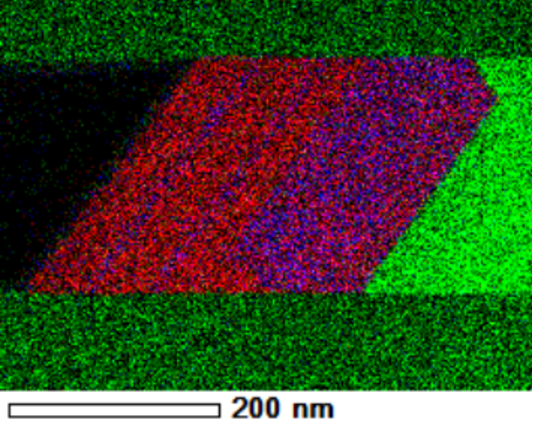
\includegraphics[width=0.45\textwidth]{3_Growth/s3_III_map.pdf}
    }
    \subcaptionbox{
        \acs{eds} map: Red-\acs{as} Green-\ce{O} Blue-\acs{p}
        \label{subfig:s3_V_map}
    }{
        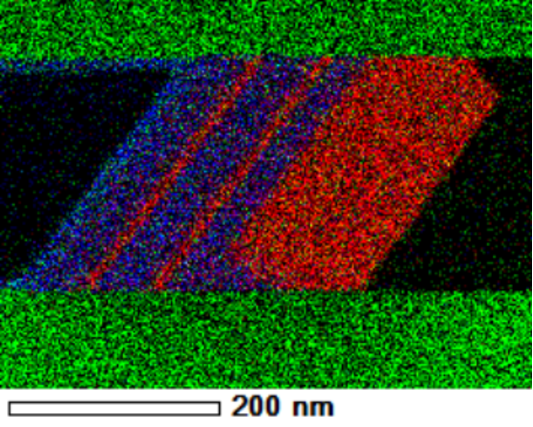
\includegraphics[width=0.45\textwidth]{3_Growth/s3_V_map.pdf}
    }
    \subcaptionbox{
        \acs{eds} map: Red-\acs{in} Blue-\acs{ga} \cite{Brugnolotto2023}
        \label{subfig:s3_III_map_wells}
    }{
        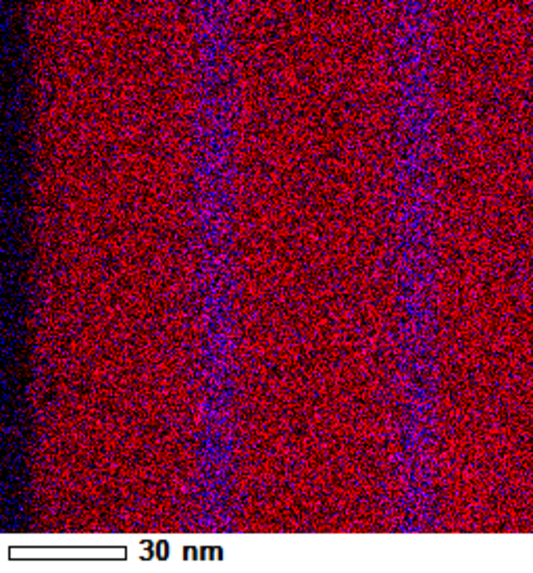
\includegraphics[width=0.45\textwidth]{3_Growth/s3_III_map_wells.pdf}
    }
    \subcaptionbox{
        \acs{eds} map: Red-\acs{as} Blue-\acs{p} \cite{Brugnolotto2023}
        \label{subfig:s3_V_map_wells}
    }{
        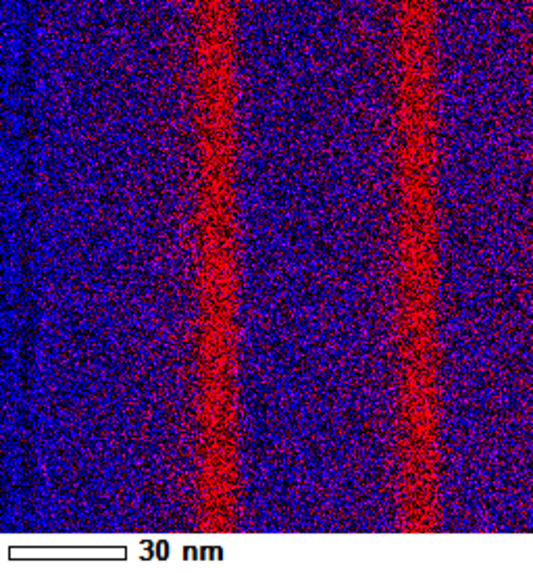
\includegraphics[width=0.45\textwidth]{3_Growth/s3_V_map_wells.pdf}
    }
    \caption[Spectroscopic analysis of sample 3.]{Spectroscopic information for sample 3. \subref{subfig:s3_III_map} and \subref{subfig:s3_V_map} are the III and V group element maps, with \acs{si} and \acs{o} to visualise the position of the seed and template. \subref{subfig:s3_III_map_wells} and \subref{subfig:s3_V_map_wells} are III and V \acs{eds} maps focussing on the superlattice region of the sample.}
    \label{fig:s3_maps}
\end{figure}

The arsenide layers in the V map are confirmed to perfectly coincide with the \acs{ga}-rich regions. However, the V map also highlights an asymmetry in the composition of the areas immediately before and after an \acs{ingaas} \acs{qw}, with the \acs{inp} region after a well showing a higher \acl{as} signal than the \acs{inp} region immediately before.

\begin{figure}
    \centering
    \subcaptionbox{
    \acs{eds} linescan: III atomic percentage vs position \cite{Brugnolotto2023}.
    \label{subfig:s3_III_linesc}
    }{
    \tikzsetnextfilename{s3_III_linesc}
    \begin{tikzpicture}
        \begin{axis}[
            width = 0.8\textwidth,
            height = 5cm,
            xlabel = Position (nm),
            ylabel = Composition (atomic \%),
            table/col sep=comma,
            %title = III group element composition,
            legend pos=outer north east,
            ymin=0, ymax=100,
            xmin = 0, xmax=20.81
        ]
    \addplot [cb1_orange,] table[x=nm,y=Ga] {3_Growth/s3_III_linesc.csv};
    \addplot [cb1_dark_blue,] table[x=nm,y=In] {3_Growth/s3_III_linesc.csv};
    \addlegendentry{Ga}
    \addlegendentry{In}
    \end{axis}

    \end{tikzpicture}
    }
    \subcaptionbox{
    \acs{eds} linescan: V atomic percentage vs position \cite{Brugnolotto2023}.
    \label{subfig:s3_V_linesc}
    }{
    \tikzsetnextfilename{s3_V_linesc}
    \begin{tikzpicture}
        \begin{axis}[
            width = 0.8\textwidth,
            height = 5cm,
            xlabel = Position (nm),
            ylabel = Composition (atomic \%),
            table/col sep=comma,
            %title = V group element composition,
            legend pos=outer north east,
            ymin=0, ymax=100,
            xmin = 0, xmax=20.81
        ]
    \addplot [cb1_orange,] table[x=nm,y=As] {3_Growth/s3_V_linesc.csv};
    \addplot [cb1_dark_blue,] table[x=nm,y=P] {3_Growth/s3_V_linesc.csv};
    \addlegendentry{As}
    \addlegendentry{P}
    \end{axis}

    \end{tikzpicture}
    }
    \caption[Composition data from an \acs{eds} linescan across a quantum well of sample 3.] {\acs{eds} linescans for the \subref{subfig:s3_III_linesc} III group elements and \subref{subfig:s3_V_linesc} V group elements across the second \acl{qw} of sample 3. The origin of the x-axis is situated before the well itself on the side of the \acs{si} seed, and higher position numbers (in nm) represent the scan moving along the \hkl{1 1 1} vector perpendicular to the growth front away from the seed.}
    \label{fig:s3_linescans}
\end{figure}

An \acs{eds} linescan was taken to quantify the composition gradient. With this methodology, the electron beam is moved point by point on a linear path instead of recording the spectra as the image is formed, as was done for the \acs{eds} maps presented so far. On each stop, a full \acs{eds} spectra is recorded; therefore, a complete compositional analysis with localised data is possible. A linescan limits the area that can be examined but, in doing so, also allows for more time to be dedicated to each measuring point, resulting in a better quantification of the sample's composition compared to the mapping method used so far.

The peak intensity of the \acl{ga} and \acl{in} L\(_\alpha\) lines (at \qty{1.098}{\kilo\eV} and \qty{3.286}{\kilo\eV}) were elaborated by the \acf{gms} to extrapolate, taking into consideration the cross section for both emission processes, the relative composition in percentage at each given survey point, resulting in the graph in Figure~\ref{subfig:s3_III_linesc}. The choice to use the L\(_\alpha\) lines of these two materials was dictated by the lack of a calibration sample and the need to use the internal parameters of the \acs{gms} software. Therefore, it was decided that the use of the same kind of line, which results from the same electronic transition, would be likely to produce more reliable results than the use of two different lines, and, while usually the K\(_\alpha\) lines would be the first choice, the \acs{in} K\(_\alpha\) line falls outside the spectral range of the \acs{eds} detector. Figure~\ref{subfig:s3_V_linesc} was generated with the same methodology, but using the \acl{as} and \acl{p} K\(_\alpha\) line at \qty{10.530}{\kilo\eV} and \qty{2.013}{\kilo\eV}, respectively, as they are both within the detector's spectral range.

The two graphs in Figure~\ref{fig:s3_linescans} show that the resulting composition profiles are very noisy, revealing the limitations of \acs{eds} with \qty{10}{\%} noise fluctuations caused by the sum of the errors in the quantification of the atomic percentages of the two elements. Despite this, specific trends can be observed, such as the presence of very little \acl{ga} in the area immediately before the \acs{ingaas} \acl{qw} in Figure~\ref{subfig:s3_III_linesc} hinting at the expected \qty{100}{\%} \acl{in} fraction for the \acs{inp} layer. The transition area for the onset of the \acs{ga}-rich well is also around \qty{2}{nm} in width, which translates to roughly \num{6} bi-atomic layers along the \hkl<1 1 1> direction. The \acs{ingaas} layer has a \ce{In0_.55Ga0_.45As} composition. Finally, in the \acs{inp} layer following the \acs{ingaas} well, there is a background \acl{ga} concentration that slowly goes down to \qty{10}{\%} at the end of the scan region.

An analysis of the atomic percentages of V group elements in the \acs{inp} barrier layers around the \acs{ingaas} well highlights a high \acl{as} background contamination. Indeed, even though before the well the \acl{as} atomic percentage is already around \qty{20}{\%}, right after the well and the transition area at the interface between the two materials, the lingering \acl{as} atomic fraction oscillates between \qty{30}{\%} and \qty{40}{\%}. In the well itself, the \acl{as} atomic percentage reaches \qty{90}{\%}. This confirms and quantifies the qualitative observation of a higher red "\acl{as}" concentration in Figure~\ref{subfig:s3_V_map_wells} immediately after the \acs{ingaas} wells. It is known that the second heterointerface of an \acs{inp}-\acs{ingaas}-\acs{inp} material stacking is not as well defined compared to the first. While this could be simply due to the reservoir effect caused by the template, which was to be avoided by the introduction of a short \acl{p} pulse before the onset of the \acs{inp} deposition step, it could also originate in decomposition mechanisms of the \acs{ingaas} known to occur in some planar deposition configurations \cite{Decobert2002}. However, if such layer degradation occurs, it is not as strong a process as observed in the literature, as the two heterointerfaces remain regular and parallel. A more detailed study of the phenomenon by changing the post-\acs{ingaas} step is required to shed light on this issue.
\par

\begin{table}
    \centering
    \caption{Growth rates for the third grown sample.}
    \begin{tabular}{l|c c c}
                               & \multicolumn{3}{c}{Growth rates (\nmmin)}                                                                                               \\
       Layer                   & \hkl<1 1 1>                                 & Longest distance                            & Shortest distance                           \\ \hline \hline
       \acs{ingaas} nucleation & \num[separate-uncertainty=true]{15.0 (0.2)} & \num[separate-uncertainty=true]{18.3 (0.2)} & \num[separate-uncertainty=true]{10.3 (0.4)} \\
       \acs{inp} stabilisation & \num[separate-uncertainty=true]{9.9 (0.3)}  & \num[separate-uncertainty=true]{34.9 (0.8)} & \num[separate-uncertainty=true]{11.7 (0.7)} \\
       \acs{ingaas} well 1     & \num[separate-uncertainty=true]{18.5 (0.5)} & N.A.                                        & N.A. \\
       \acs{inp} barrier 1     & \num[separate-uncertainty=true]{13.7 (0.2)} & N.A.                                        & N.A. \\ 
       \acs{ingaas} well 2     & \num[separate-uncertainty=true]{17 (1)}     & N.A.                                        & N.A. \\
       \acs{inp} barrier 2     & \num[separate-uncertainty=true]{13.9 (0.1)} & N.A.                                        & N.A. \\ \hline
    \end{tabular}
    \label{tab:sample3_growth_rates}
\end{table}

\paragraph{Growth metrics} Table~\ref{tab:sample3_growth_rates} shows the growth rates for the different material layers in the sample, measured the same way as for those in Table~\ref{tab:sample1_growth_rates}. The three ways of measuring growth rates were used for the first two layers: the \acs{ingaas} nucleation layer and the \acs{inp} stabilisation layer (named after its role in stabilising a single \hkl{1 1 1} facet as the growth front). As the single-facet growth front is established, the \hkl<1 1 1> growth rates become the actual growth rate of the wire and, therefore, only it is given for the remaining four layers. 

Having access to the information regarding the growth rates of each material in both a single- and multi-facet growth front allows us to analyse the effect of each growth configuration. Both the \hkl<1 1 1> growth rates for the first \acs{ingaas} and \acs{inp} layers are lower than those after the growth front is stabilised. While for the nucleation layer this is likely due to the need for the initial crystal to expand and fill the template, for the \acs{inp} stabilisation layer this is mainly due to the rapid annihilation of the \hkl{1 1 0} facet, as is made evident by the high "longest distance" growth rate, which is measured along the \hkl<1 1 0> template axis at the bottom of the corresponding \acs{inp} segment in Figure~\ref{fig:s3_ov}.

The growth rates differ significantly from those in Table~\ref{tab:sample1_growth_rates} for the \acs{ingaas} layer. This could be due to the different morphology of the growth front, which has a much larger \hkl{1 1 1} facet. For the \acs{inp} layer, on the other hand, the growth rates remained somewhat comparable. The \hkl<1 1 1> growth rate is higher, however, which could be explained by the smaller \hkl<1 1 0> facet having to be filled after the \acs{ingaas} layer. This is also reflected in the lower growth rate for the \hkl<1 1 0> template axis "long direction".

After the stabilisation layer, the growth rates of the two wells and those of the two barriers are comparable and within each other's uncertainty interval.
\par

\section{Discussion and future developments}

The main accomplishment in this chapter was the identification and exploitation of the high V/III ratio \acs{inp} \acs{mocvd} growth conditions' effect on the stabilisation of the \hkl{1 1 1}\(_B\) facet as the single growth front for the growing III-V nanowire. This avoids issues related to different incorporation rates of III group elements in ternary materials such as \acs{ingaas} \cite{Borg2019} and creates compositionally uniform material layers. This is then united with the introduction of hold steps, which mitigate the effect of the adsorbate diffusion pathway, avoiding creating a reservoir effect for the III-component, which are integrated into their design layer as expected and without delay. 

This is expected to provide a solution or, at the very least, improve on all of the issues identified in Figure~\ref{fig:wen}. However, some critical problems remain. The first is related to the possibility of the stabilisation of either of 2 different \hkl{1 1 1} facets. This negates the advantage gained in terms of contact positioning, as the selection of the \hkl{1 1 1} facet remains a stochastic process. This is an unsolvable problem with the \hkl[0 0 1] \acs{soi} wafer, as this substrate defines the crystalline orientation of the growing wire. 

As the experiments described on this sample were being carried out, Markus F. Ritter was in the process of publishing a paper on hybrid \acs{tase}, a methodology through which part of the \acs{sio2} template is switched out for a superconducting material \cite{Ritter2021}. As a result of a collaboration on the \acs{stem_m} analysis of hybrid \acs{tase} samples, access to \hkl[1 1 0] \acs{soi} wafers as a growth substrate was obtained for this project. This new crystalline orientation of the growth substrate means that there are in-plane \hkl<1 1 1> vectors at high angles with respect to each other, and prompted my interest in using these wafers as the substrate for the next steps of my research.

This new wafer had a \acl{si} device layer thickness of \qty{70}{\nano\metre} and a \qty{220}{\nano\metre}-thick buried oxide layer, compared to the \hkl[0 0 1] wafer employed so far for which the thicknesses were \qty{220}{\nano\metre} and \qty{2}{\micro\metre}, respectively. The new wafer, therefore, is less suited for optoelectronic and photonic applications but should still prove an ideal test bed for the study of \acs{mocvd} growth dynamics.

In particular, there are remaining questions on the reproducibility of the study, the yield of the growth stabilization, the optical properties of the devices and the application of this facet stabilization method to the integration of different III-V materials outside of the lattice-matched \ce{In0_.55Ga0_.45As} and \acs{inp} material system \cite{Pearsall1980, Sugii1983, Wagner1970} studied in this chapter.